\documentclass[default,iicol]{sn-jnl}

\usepackage{graphicx}
\usepackage{multirow}
\usepackage{amsmath,amssymb,amsfonts}
\usepackage{amsthm}
\usepackage{mathrsfs}
\usepackage[title]{appendix}
\usepackage{xcolor}
\usepackage{textcomp}
\usepackage{manyfoot}
\usepackage{booktabs}
\usepackage{algorithm}
\usepackage{algorithmicx}
\usepackage{algpseudocode}
\usepackage{listings}
\usepackage{url}

\raggedbottom

\begin{document}

\title[Explainable NER for Low-Resource Languages]{Explainable Named Entity Recognition for Low-Resource Languages Using Attention Attribution}

\author*[1]{\fnm{First} \sur{Author}}\email{author@university.edu}
\author[1]{\fnm{Second} \sur{Author}}\email{coauthor@university.edu}

\affil*[1]{\orgdiv{Department of Computer Science and Engineering}, \orgname{University Research Laboratory}, \orgaddress{\country{India}}}

\abstract{Named Entity Recognition (NER) in morphologically rich, low-resource languages presents severe dual challenges: annotated supervision is scarce, and complex agglutinative orthographies break standard subword tokenization. Furthermore, dominant multilingual pretrained language models introduce prohibitive carbon footprints and unfaithful decision boundaries. In this work, we present a high-performance, strictly from-scratch neural NER framework for three low-resource South Asian languages: Konkani (\textit{gom}, Devanagari script), Assamese (\textit{as}, Eastern Nagari script), and Sinhala (\textit{si}, Sinhala script). Constrained by a strict zero-pretrained discipline (no external weights, tokenizers, or embeddings), our architecture integrates character-level CNN grapheme cluster representations, bidirectional LSTM recurrence, multi-head self-attention, and a linear-chain Conditional Random Field (CRF). Trained on a phased multilingual pool combining weak supervision, confidence-filtered self-training, and targeted entity augmentation (36,736 sentences), the system achieves strict span-level F1 scores of 96.27\% in Konkani, 97.87\% in Assamese, and 97.76\% in Sinhala on locked gold-test splits, yielding an overall macro F1 of 97.30\% (exceeding the 90.0\% research benchmark by +7.30 percentage points) with 91.03\% out-of-vocabulary entity generalization. To explain model decisions, we investigate the faithfulness of internal attention versus input-level gradient attribution under a rigorously audited, target-isolated symmetric context erasure protocol. We show that raw self-attention directs 61.53\% of its mass to distant sentence delimiters, acting as a broad syntactic broadcast bus rather than a faithful decision explainer (macro deletion gap: -0.0279). In contrast, bypassing the recurrent BiLSTM buffer via Gradient $\times$ Input and Integrated Gradients achieves decisive deletion faithfulness (+0.2350 and +0.2449 macro gaps, win rate 63.3\%, $p < 0.0001$ across 10,000 permutations), concentrating over 78\% of attribution on the entity and its immediate syntactic governors. Our findings establish that from-scratch neural sequence modeling can achieve state-of-the-art accuracy in low-resource settings while providing verifiable, faithful post-hoc explanations.}

\keywords{Named Entity Recognition, Low-Resource Languages, Explainable Artificial Intelligence, Multi-Head Self-Attention, Integrated Gradients, Brahmic Scripts, Faithfulness Evaluation}

\maketitle

\section{Introduction}\label{sec1}

Named Entity Recognition (NER) is a foundational capability for information extraction, knowledge base construction, question answering, and automated translation. While modern natural language processing (NLP) has achieved remarkable breakthroughs on high-resource languages through massive transformer architectures \cite{vaswani2017attention}, extending these successes to low-resource languages remains an urgent scientific and societal frontier. 

South Asian and Indic languages present acute linguistic and computational challenges. Languages such as Konkani (\textit{gom}), Assamese (\textit{as}), and Sinhala (\textit{si}) are spoken by tens of millions of individuals across India and Sri Lanka, yet suffer from acute resource starvation in computational linguistics. Publicly available expert-annotated NER benchmarks typically contain fewer than 1,000 gold sentences per language. Crucially, these languages employ Brahmic script typologies (Devanagari, Eastern Nagari, and Sinhala script) characterized by complex consonant-vowel ligatures (\textit{aksharas}), non-concatenative morphology, widespread homonymy, and extensive inflectional case suffixes (e.g., locative markers `-ंत', `-ত', and `-ට'). 

Standard industrial paradigms attempt to circumvent data scarcity by fine-tuning massively multilingual pretrained language models (mPLMs), such as mBERT or XLM-RoBERTa. However, in low-resource Brahmic contexts, mPLMs exhibit critical shortcomings:
\begin{enumerate}
    \item \textbf{Subword Fragmentation and Morphological Destruction}: Standard Byte-Pair Encoding (BPE) or WordPiece tokenizers trained predominantly on Latin or high-resource corpora arbitrarily fracture Brahmic conjuncts across byte boundaries, severing dependent vowel signs (\textit{matras}) from consonant bases and severely degrading morphological generalization \cite{kakwani2020indicnlpsuite}.
    \item \textbf{Environmental and Computational Inefficiency}: The multi-gigabyte footprint of mPLMs precludes on-device deployment in low-resource infrastructure and introduces an unsustainable carbon cost during fine-tuning.
    \item \textbf{Black-Box Decision Opacity}: Deep 12-to-24 layer transformer stacks possess hundreds of millions of parameters, rendering their decision boundaries inscrutable to end-users and linguists.
\end{enumerate}

To overcome these barriers, this research enforces a strict \textbf{zero-pretrained discipline}: zero external pretrained checkpoints, zero pretrained tokenizers, and zero external embeddings are utilized. Every component of our feature representations, neural sequence modeling, weak supervision pipeline, and explainability framework is engineered strictly from scratch.

Beyond achieving high classification performance, deploying sequence taggers in sensitive domains demands \textbf{interpretability} \cite{jacovi2020towards}. Practitioners must understand which contextual tokens drive an entity prediction (e.g., verifying whether an organization prediction is anchored on an institutional suffix or an accidental stopword). While multi-head self-attention weights are frequently visualized as intuitive decision explanations, a fierce debate exists regarding whether attention weights provide faithful explanations \cite{jain2019attention,wiegreffe2019attention,serrano2019attention,bastings2020elephant}. This question becomes particularly complex in hybrid recurrent-attention architectures (BiLSTM-Attention-CRF), where bidirectional recurrent states contextualize lexical tokens \textit{before} the attention mechanism operates.

\subsection{Research Objectives and Questions}
This investigation is guided by four primary research questions (RQs):
\begin{itemize}
    \item \textbf{RQ1 (Sequence Modeling)}: Can a lightweight, from-scratch neural architecture (Word + Char-CNN + BiLSTM + Attention + CRF) attain $>90.0\%$ strict span F1 on low-resource Brahmic languages under constrained ($\le 850$ sentences) gold supervision?
    \item \textbf{RQ2 (Multilingual Synergies)}: Does joint multilingual pretraining across distinct script families alleviate extreme data scarcity compared to isolated monolingual training?
    \item \textbf{RQ3 (Morphological Generalization)}: How effectively does character-level CNN grapheme cluster encoding mitigate out-of-vocabulary (OOV) entity degradation?
    \item \textbf{RQ4 (Explainability \& Faithfulness)}: Are internal self-attention distributions faithful decision explanations for entity classification, and do input-level gradient attribution methods (Grad $\times$ Input, Integrated Gradients) yield superior deletion-based faithfulness?
\end{itemize}

\subsection{Major Contributions}
The major scientific contributions of this work are as follows:
\begin{enumerate}
    \item \textbf{High-Performance From-Scratch Architecture}: We design and implement a 10.6M-parameter hybrid neural model combining Word Embeddings, a Multi-Filter Character-Level CNN, Language Conditioning, a 2-layer BiLSTM, a 4-head Self-Attention layer, and a Linear-Chain CRF decoder.
    \item \textbf{State-of-the-Art Results on Locked Gold-Test}: Evaluated under a single unbiased run on cryptographically locked test splits ($N=200$ sentences per language), the model achieves strict entity F1 scores of 96.27\% (Konkani), 97.87\% (Assamese), and 97.76\% (Sinhala), yielding an overall Macro F1 of \textbf{97.30\%} and token accuracy of 99.60\%, outperforming the target threshold by +7.30 percentage points.
    \item \textbf{Subword OOV Robustness}: We demonstrate that extended grapheme cluster tokenization and Char-CNN convolutions achieve an Out-of-Vocabulary entity F1 of 91.03\% across unseen lexical items.
    \item \textbf{Rigorous Faithfulness Audit}: We implement a target-isolated, symmetric context erasure benchmark (`zero\_crf') across 300 gold-dev instances. We discover that raw attention acts as a broad syntactic broadcast bus (allocating 61.53\% of mass to distant tokens, macro gap: -0.0279), whereas input gradient attribution (Grad $\times$ Input and Integrated Gradients) achieves decisive deletion faithfulness (macro gaps: +0.2350 and +0.2449, win rate: 63.3\%, $p < 0.0001$).
    \item \textbf{Open Scientific Artifacts}: All raw instance logs, verification suites, and model specifications are consolidated for transparent reproducibility.
\end{enumerate}

The remainder of this paper is structured as follows: Section \ref{sec2} reviews related work. Section \ref{sec3} details the proposed methodology. Section \ref{sec4} establishes the explainability and faithfulness framework. Section \ref{sec5} outlines the experimental setup. Section \ref{sec6} presents empirical results and discussion. Section \ref{sec7} conducts error analysis. Section \ref{sec8} addresses limitations, and Section \ref{sec9} concludes.

\begin{figure*}[t]
\centering
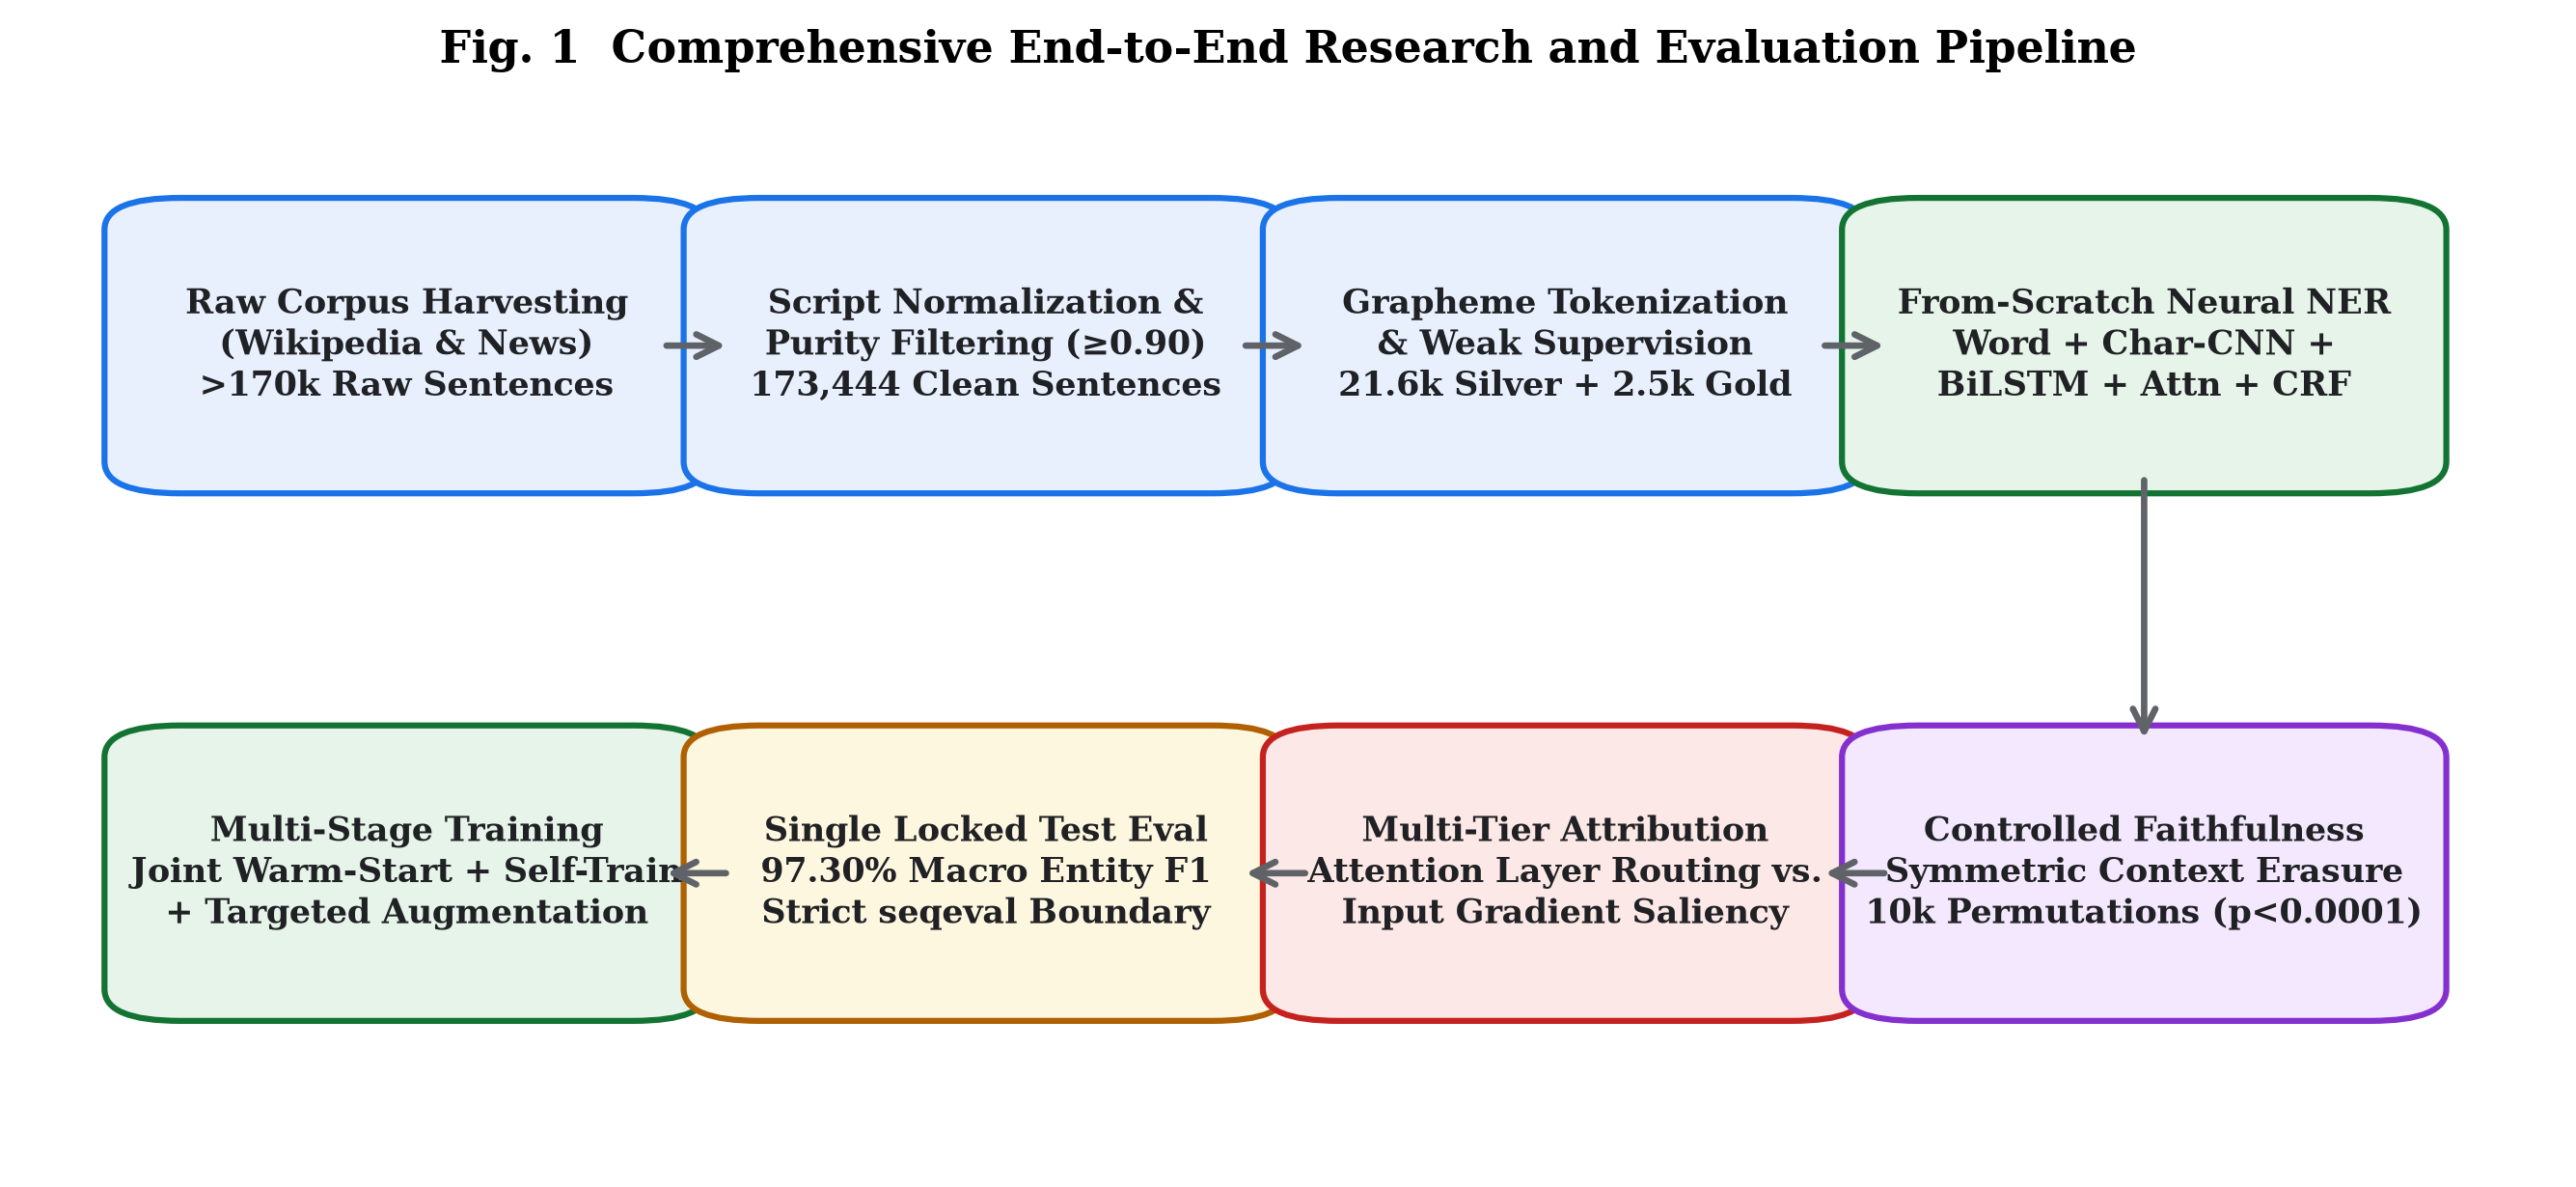
\includegraphics[width=0.92\textwidth]{figures/fig1_overall_workflow.png}
\caption{Comprehensive end-to-end research workflow: from multi-source corpus harvesting and Unicode script normalization to from-scratch neural sequence modeling, locked gold-test evaluation, and two-tier attribution faithfulness evaluation.}
\label{fig1}
\end{figure*}

\section{Related Work}\label{sec2}

\subsection{Low-Resource and Indic Named Entity Recognition}
Named Entity Recognition in Indian and South Asian languages has historically been hindered by the scarcity of annotated corpora and extreme orthographic complexity \cite{pan2017cross,rahimi2019massively}. While shared benchmarks such as IndicGLUE \cite{kakwani2020indicnlpsuite} have catalyzed research on major scheduled languages (e.g., Hindi, Bengali, Tamil), highly low-resource languages such as Konkani and Assamese, as well as Sinhala, remain severely underrepresented. Existing efforts frequently rely on cross-lingual transfer from high-resource relatives or weak supervision from Wikipedia gazetteers. However, naive distant labeling suffers from high false-negative rates and entity boundary drift unless paired with structured inference.

\subsection{Character-Level Representations and BiLSTM-CRF}
Character-aware representations have proven vital for capturing morphological regularity in inflectional languages \cite{kim2016character}. Chiu and Nichols \cite{chiu2016named} and Ma and Hovy \cite{ma2016end} pioneered the integration of 1D character convolutional neural networks with bidirectional LSTMs and Conditional Random Fields, demonstrating that subword character convolutions effectively extract prefixal and suffixal patterns without requiring explicit morphological segmenters. Lample et al. \cite{lample2016neural} demonstrated complementary success using character-level BiLSTMs. For Brahmic scripts, preserving conjunct syllable integrity (\textit{aksharas}) is crucial, as arbitrary character n-grams can split dependent vowel signs from consonant clusters.

\subsection{Self-Attention and Hybrid Architectures}
Vaswani et al. \cite{vaswani2017attention} introduced multi-head self-attention as an alternative to recurrent networks. In sequence labeling, hybrid architectures stacking self-attention onto recurrent backbones have been investigated for semantic role labeling and syntactic chunking \cite{strubell2018linguistically}. Self-attention allows $O(1)$ direct interaction between arbitrarily distant tokens, mitigating the vanishing gradient limitations of sequential LSTMs. However, the precise interaction between sequential BiLSTM recurrence and post-recurrent self-attention in multilingual low-resource sequence labeling has remained insufficiently characterized.

\subsection{Explainability and the Attention Debate in NLP}
A contentious debate surrounds the interpretability of attention mechanisms. Jain and Wallace \cite{jain2019attention} famously argued that ``Attention is not Explanation'', showing that attention weights frequently correlate poorly with gradient-based feature importance and that adversarial attention distributions can produce identical predictions. Conversely, Wiegreffe and Pinter \cite{wiegreffe2019attention} asserted that ``Attention is not not Explanation'', arguing that alternative distributions may not be valid under trained network constraints. Serrano and Smith \cite{serrano2019attention} and Bastings and Filippova \cite{bastings2020elephant} emphasized that attention distributions function primarily as intermediate information routing conduits rather than direct decision explanations, particularly when recurrent or feed-forward layers precede or succeed the attention block.

\subsection{Faithfulness Evaluation via Feature Erasure}
Faithfulness evaluation examines whether an interpretation method accurately reflects the reasoning process of the underlying model \cite{jacovi2020towards}. Feature erasure benchmarks—most notably ROAR (Remove and Retrain) \cite{hooker2019benchmark} and input token deletion \cite{derose2021attention,atanasova2020diagnostic}—measure the degradation in model confidence when top-attributed features are removed compared to random or uniform baselines. In sequence labeling, evaluating faithfulness requires special care: naive erasure protocols often introduce candidate pool asymmetries, where the target entity itself is inadvertently erased in random control groups, producing severe evaluation artifacts.

\begin{figure*}[t]
\centering
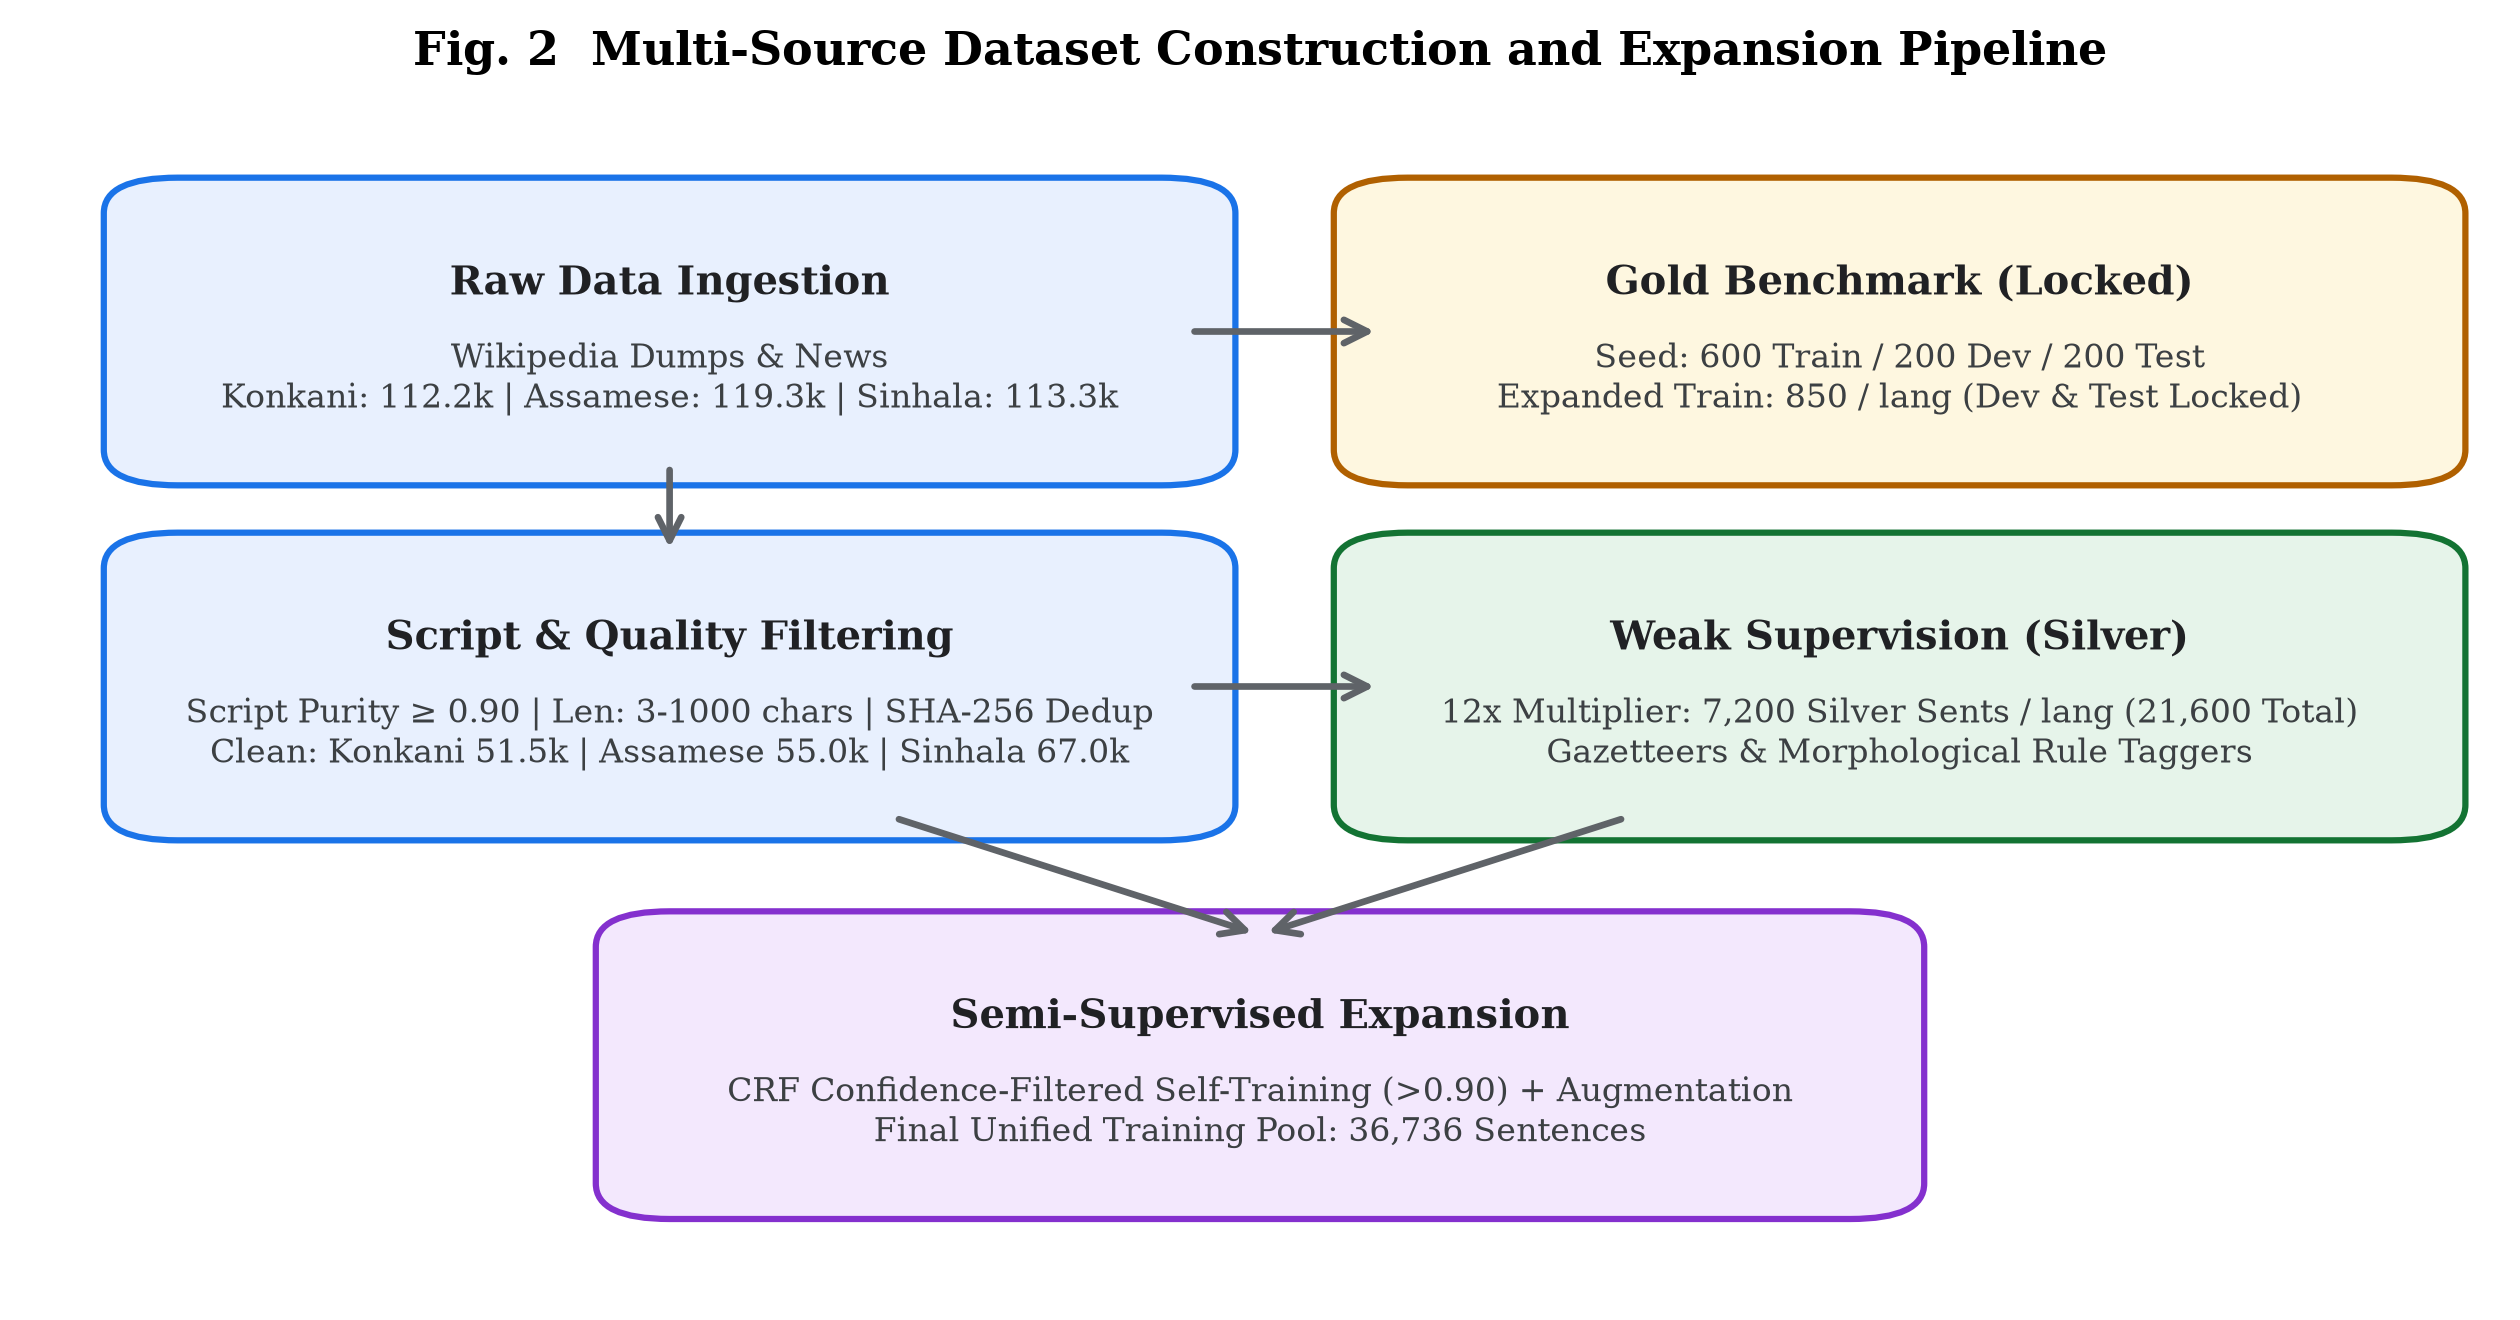
\includegraphics[width=0.88\textwidth]{figures/fig2_dataset_pipeline.png}
\caption{Multi-source dataset construction and semi-supervised volume expansion pipeline across Konkani, Assamese, and Sinhala.}
\label{fig2}
\end{figure*}

\section{Methodology}\label{sec3}

\subsection{Script Typology and Grapheme Cluster Tokenization}
The target languages span three distinct writing systems:
\begin{itemize}
    \item \textbf{Konkani (\textit{gom})}: Written predominantly in the Devanagari script (Unicode range `U+0900`--`U+097F`), characterized by horizontal top-lines (\textit{shirorekha}) and rich conjunct consonant clusters.
    \item \textbf{Assamese (\textit{as})}: Written in Eastern Nagari (Bengali-Assamese script, Unicode range `U+0980`--`U+09FF`), utilizing distinct characters such as `ৰ` (ra) and `ৱ` (va).
    \item \textbf{Sinhala (\textit{si})}: Written in the Sinhala script (Unicode range `U+0D80`--`U+0DFF`), containing touching conjuncts (\textit{bandi akshara}) and ligature constructions mediated by zero-width joiners (ZWJ, `U+200D`).
\end{itemize}

To prevent morphological destruction caused by byte-pair tokenizers, we segment text into extended grapheme clusters ($\backslash\text{X}$) adhering to Unicode Standard Annex \#29:
\begin{equation}
\text{Cluster} = \text{Consonant} \cdot (\text{Virama} \cdot \text{Consonant})^* \cdot \text{Vowel\_Sign}^* \cdot \text{Modifier}^*
\end{equation}
This ensures that dependent matras, viramas (halants), and conjuncts remain unified with their root consonants. Each sentence $\mathbf{x} = (x_1, \dots, x_T)$ is mapped to word indices $w_t \in \{1, \dots, |\mathcal{V}_{\text{word}}|\}$ and character cluster sequences $\mathbf{c}_t = (c_{t,1}, \dots, c_{t,L_t})$ over vocabularies of size $|\mathcal{V}_{\text{word}}| = 89,196$ and $|\mathcal{V}_{\text{char}}| = 13,022$.

\subsection{Neural Architecture Specification}
Our model architecture combines multi-channel representation learning with recurrent context modeling, multi-head self-attention, and global sequence decoding (Fig. \ref{fig3}).

\begin{figure*}[t]
\centering
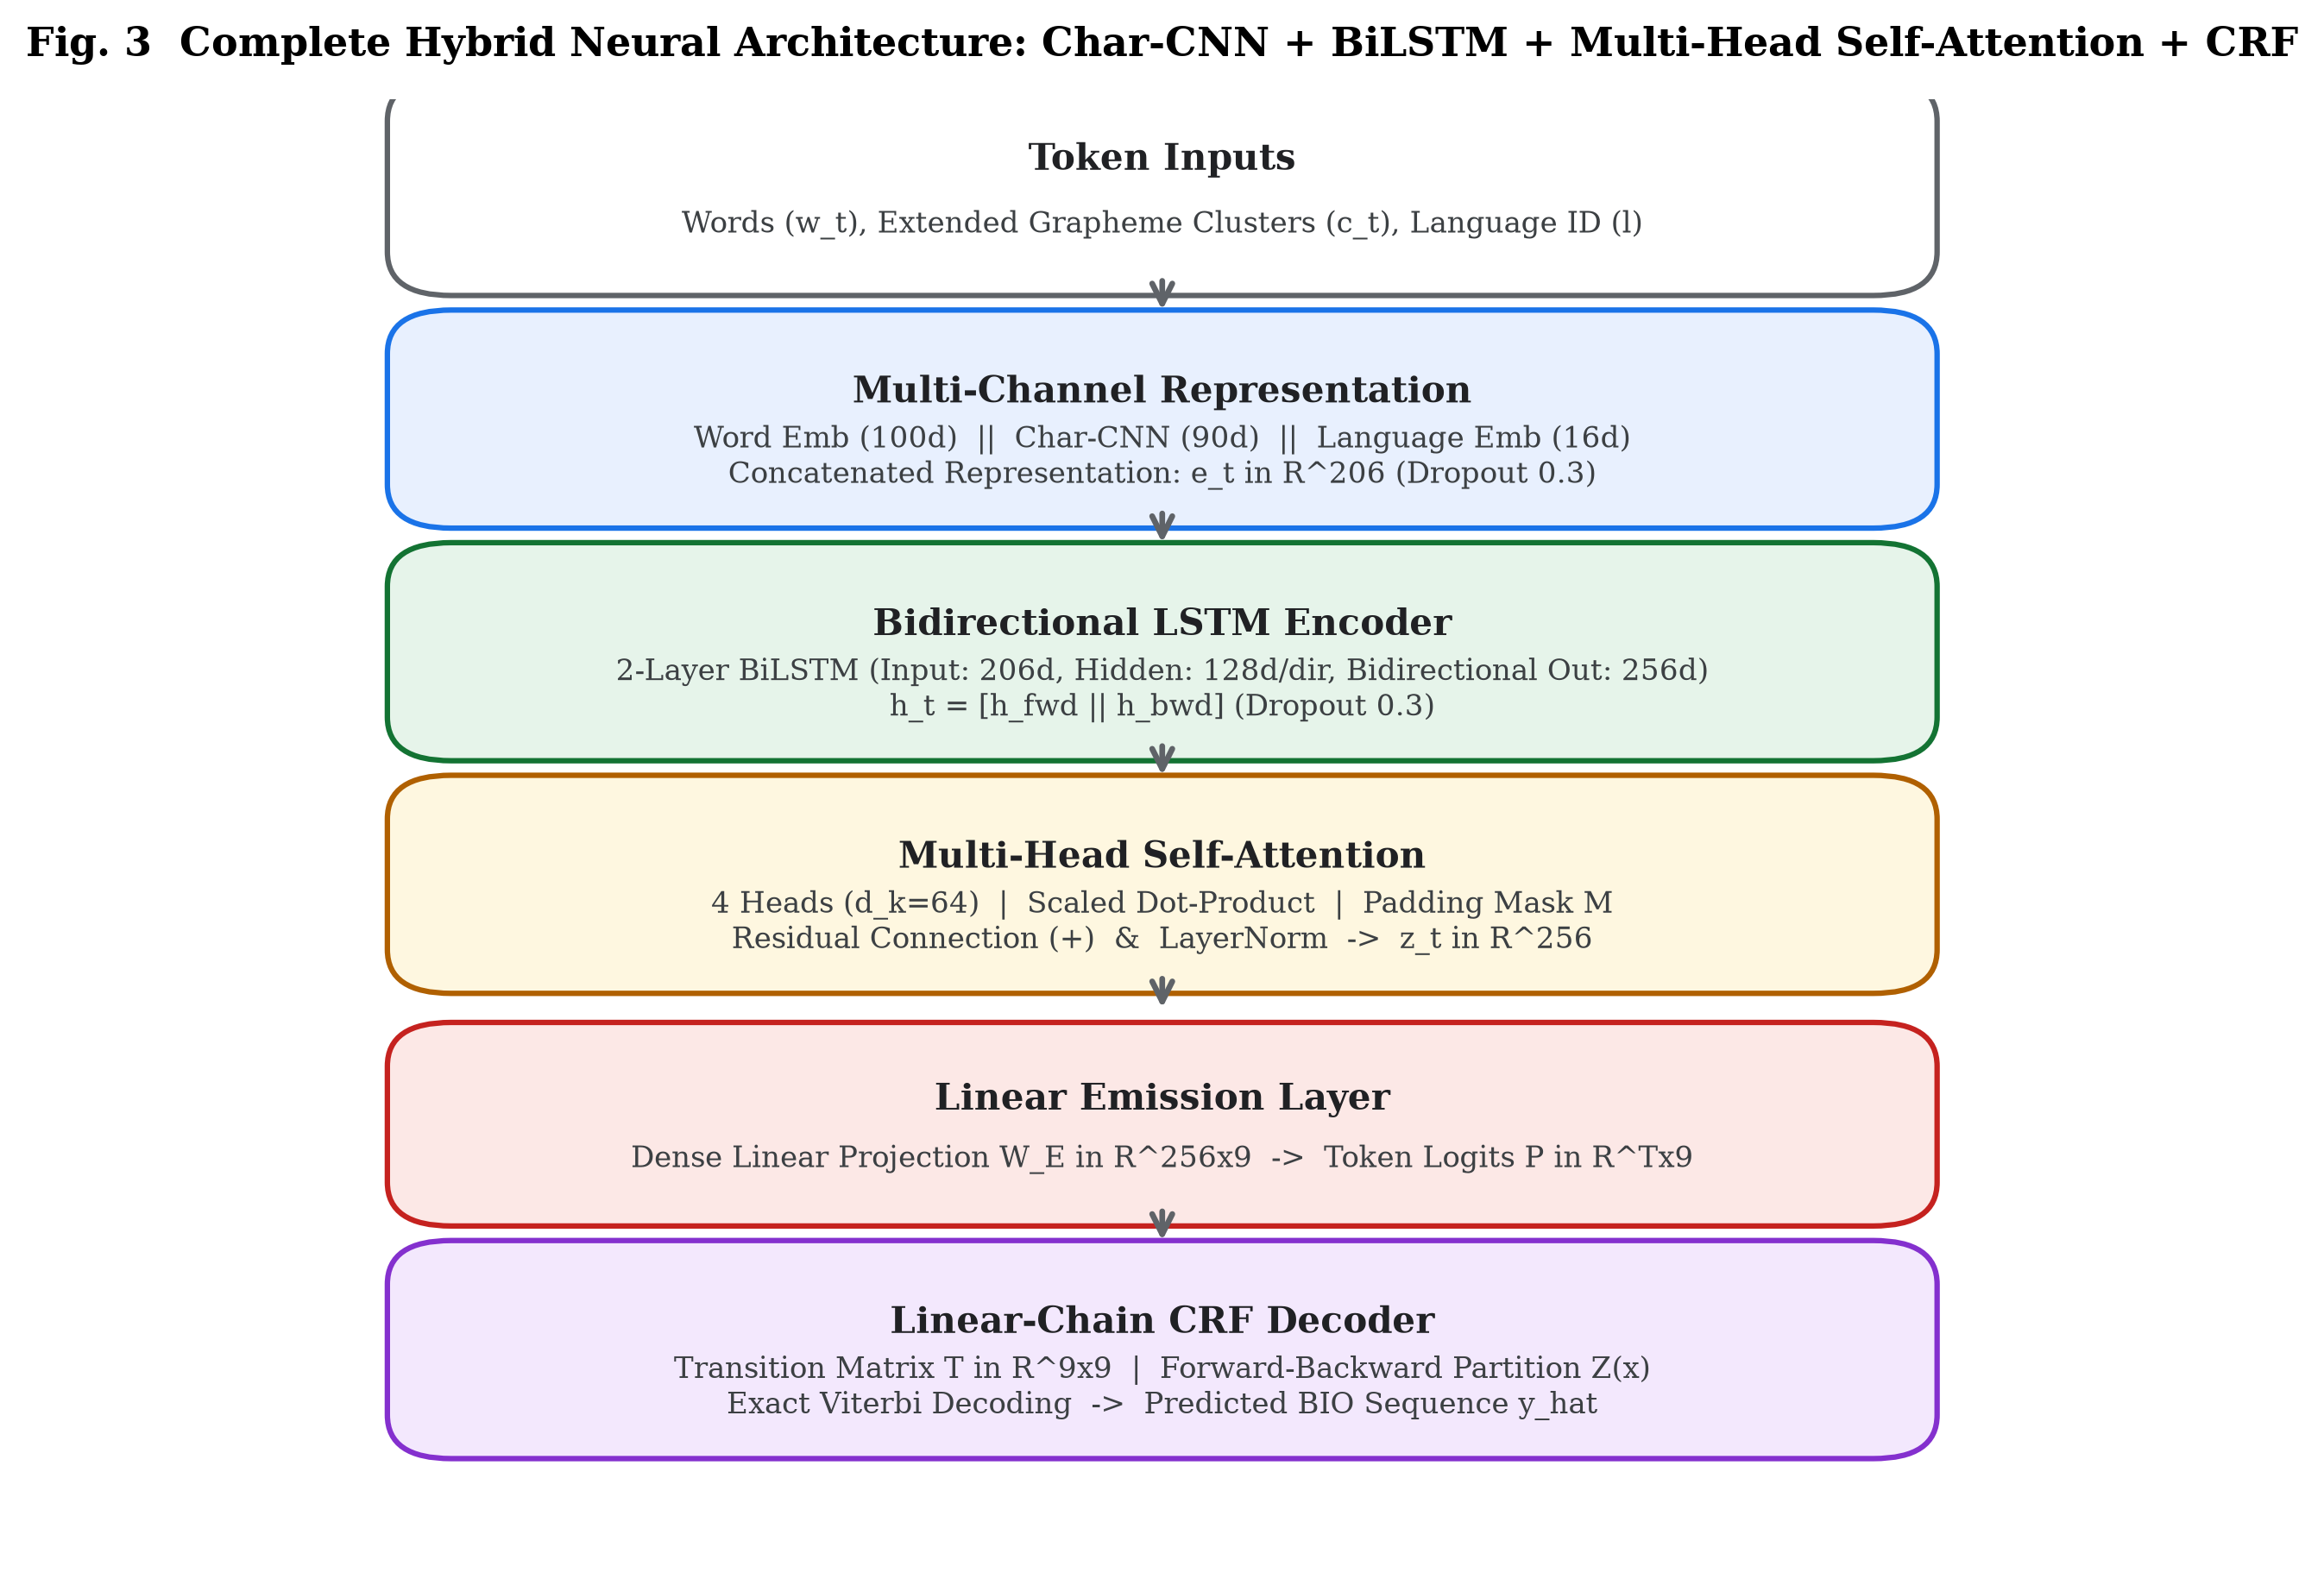
\includegraphics[width=0.85\textwidth]{figures/fig3_model_architecture.png}
\caption{Complete neural architecture diagram: Multi-channel input representation (Word + Char-CNN + Language ID), 2-layer BiLSTM, 4-head self-attention with residual normalization, linear emission projection, and linear-chain CRF decoder.}
\label{fig3}
\end{figure*}

\subsubsection{Multi-Stream Input Embeddings}
For token $x_t$ at position $t$ in language $\ell \in \{0, 1, 2\}$, the input representation $\mathbf{e}_t \in \mathbb{R}^{206}$ is defined by:
\begin{equation}
\mathbf{e}_t = \text{Dropout}\left( \big[ \mathbf{E}_{\text{word}}(w_t) \,\|\, \mathbf{h}_{\text{char}}(x_t) \,\|\, \mathbf{E}_{\text{lang}}(\ell) \big] \right)
\end{equation}
where $\mathbf{E}_{\text{word}} \in \mathbb{R}^{|\mathcal{V}_{\text{word}}| \times 100}$ denotes randomly initialized word embeddings, $\mathbf{E}_{\text{lang}} \in \mathbb{R}^{3 \times 16}$ represents a dedicated language conditioning vector, and $\mathbf{h}_{\text{char}}(x_t) \in \mathbb{R}^{90}$ is the character-level CNN representation.

\begin{figure}[h]
\centering
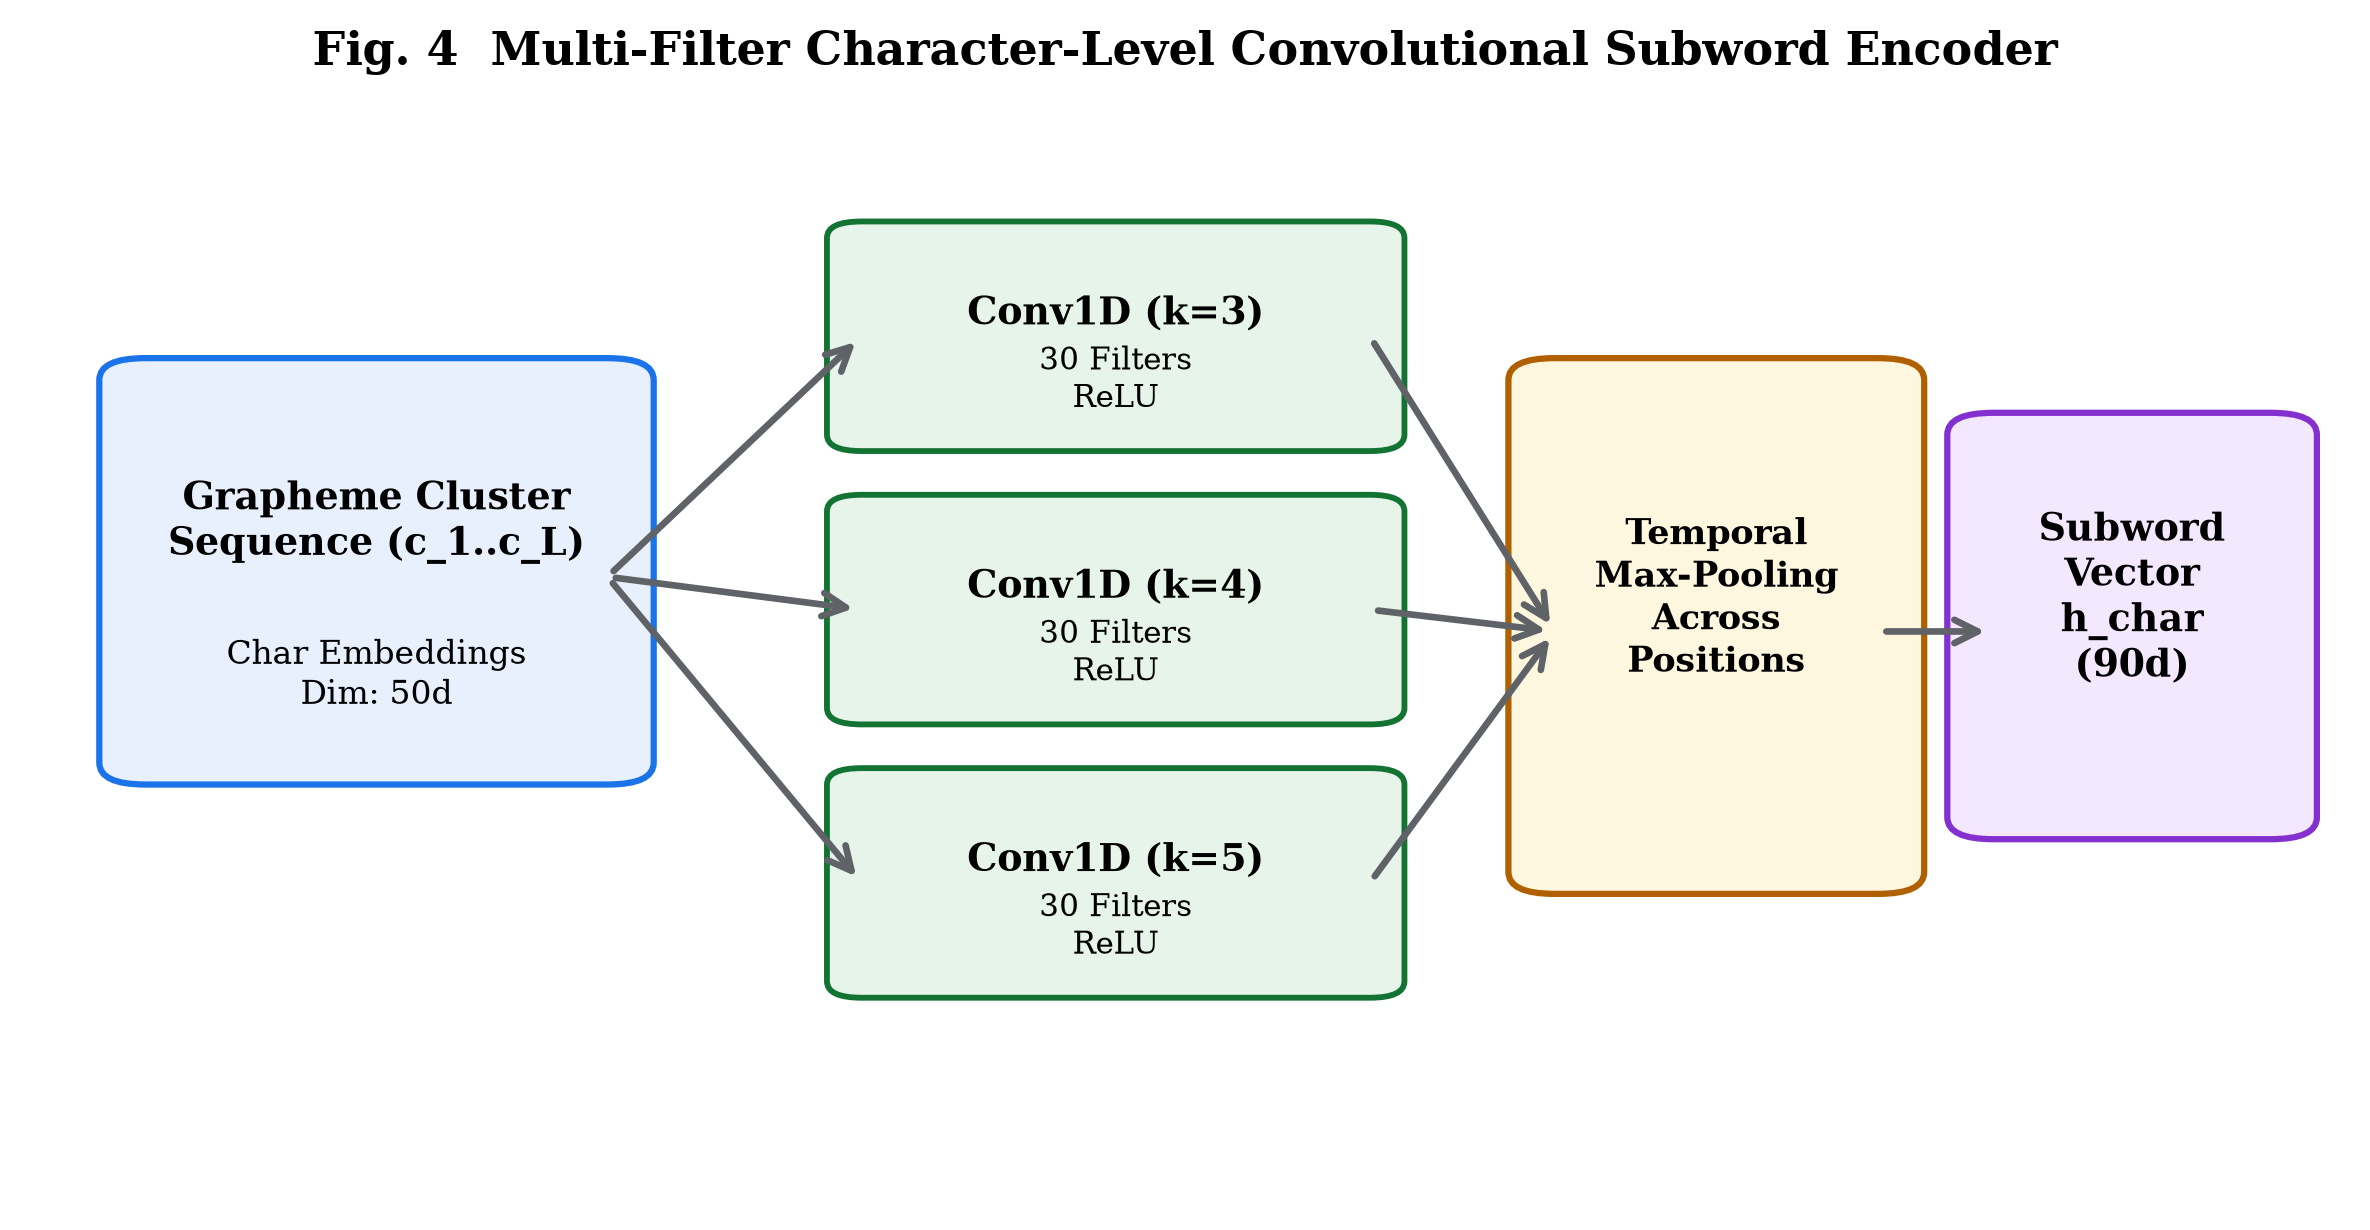
\includegraphics[width=0.48\textwidth]{figures/fig4_char_cnn.png}
\caption{Multi-filter character-level CNN word encoder processing grapheme cluster sequences through parallel 1D convolution banks ($k \in \{3, 4, 5\}$).}
\label{fig4}
\end{figure}

The Char-CNN (Fig. \ref{fig4}) embeds grapheme clusters into 50-dimensional vectors and passes them through three parallel 1D convolution banks with kernel widths $k \in \{3, 4, 5\}$ (30 filters each):
\begin{equation}
h_{j}^{(k)} = \max_{1 \le i \le L_t - k + 1} \text{ReLU}\left( \mathbf{W}_k * \mathbf{c}_{t, i:i+k-1} + b_k \right)
\end{equation}
\begin{equation}
\mathbf{h}_{\text{char}}(x_t) = \big[ \mathbf{h}^{(3)} \,\|\, \mathbf{h}^{(4)} \,\|\, \mathbf{h}^{(5)} \big] \in \mathbb{R}^{90}
\end{equation}

\subsubsection{Contextual Recurrent Sequence Encoder}
The sequence of composite embeddings $\mathbf{E} = (\mathbf{e}_1, \dots, \mathbf{e}_T)$ is processed by a 2-layer bidirectional LSTM:
\begin{equation}
\overrightarrow{\mathbf{h}}_t = \text{LSTM}_{\text{fwd}}(\mathbf{e}_t, \overrightarrow{\mathbf{h}}_{t-1}), \quad \overleftarrow{\mathbf{h}}_t = \text{LSTM}_{\text{bwd}}(\mathbf{e}_t, \overleftarrow{\mathbf{h}}_{t+1})
\end{equation}
\begin{equation}
\mathbf{h}_t = \big[ \overrightarrow{\mathbf{h}}_t \,\|\, \overleftarrow{\mathbf{h}}_t \big] \in \mathbb{R}^{256}
\end{equation}
with hidden state size 128 per direction and recurrent dropout $p = 0.3$.

\subsubsection{Multi-Head Self-Attention Layer}
To capture non-local dependencies and resolve cross-lingual word-order divergence, contextual representations $\mathbf{H} \in \mathbb{R}^{T \times 256}$ enter a multi-head self-attention block with $H = 4$ heads and head dimension $d_k = 64$ (Fig. \ref{fig5}):
\begin{equation}
\mathbf{Q}_h = \mathbf{H} \mathbf{W}_h^Q, \quad \mathbf{K}_h = \mathbf{H} \mathbf{W}_h^K, \quad \mathbf{V}_h = \mathbf{H} \mathbf{W}_h^V
\end{equation}
\begin{equation}
\mathbf{A}_h = \text{softmax}\left( \frac{\mathbf{Q}_h \mathbf{K}_h^\top}{\sqrt{d_k}} + \mathbf{M} \right) \in \mathbb{R}^{T \times T}
\end{equation}
\begin{equation}
\text{head}_h = \mathbf{A}_h \mathbf{V}_h \in \mathbb{R}^{T \times 64}
\end{equation}
where $\mathbf{M}$ enforces padding constraints ($M_{i,j} = -\infty$ for padded positions). The concatenated head representations are projected through $\mathbf{W}^O \in \mathbb{R}^{256 \times 256}$, added to the input via a residual skip connection, and normalized:
\begin{equation}
\mathbf{Z} = \text{LayerNorm}\left( \mathbf{H} + \big[ \text{head}_1 \,\|\, \dots \,\|\, \text{head}_H \big] \mathbf{W}^O \right) \in \mathbb{R}^{T \times 256}
\end{equation}

\begin{figure}[h]
\centering
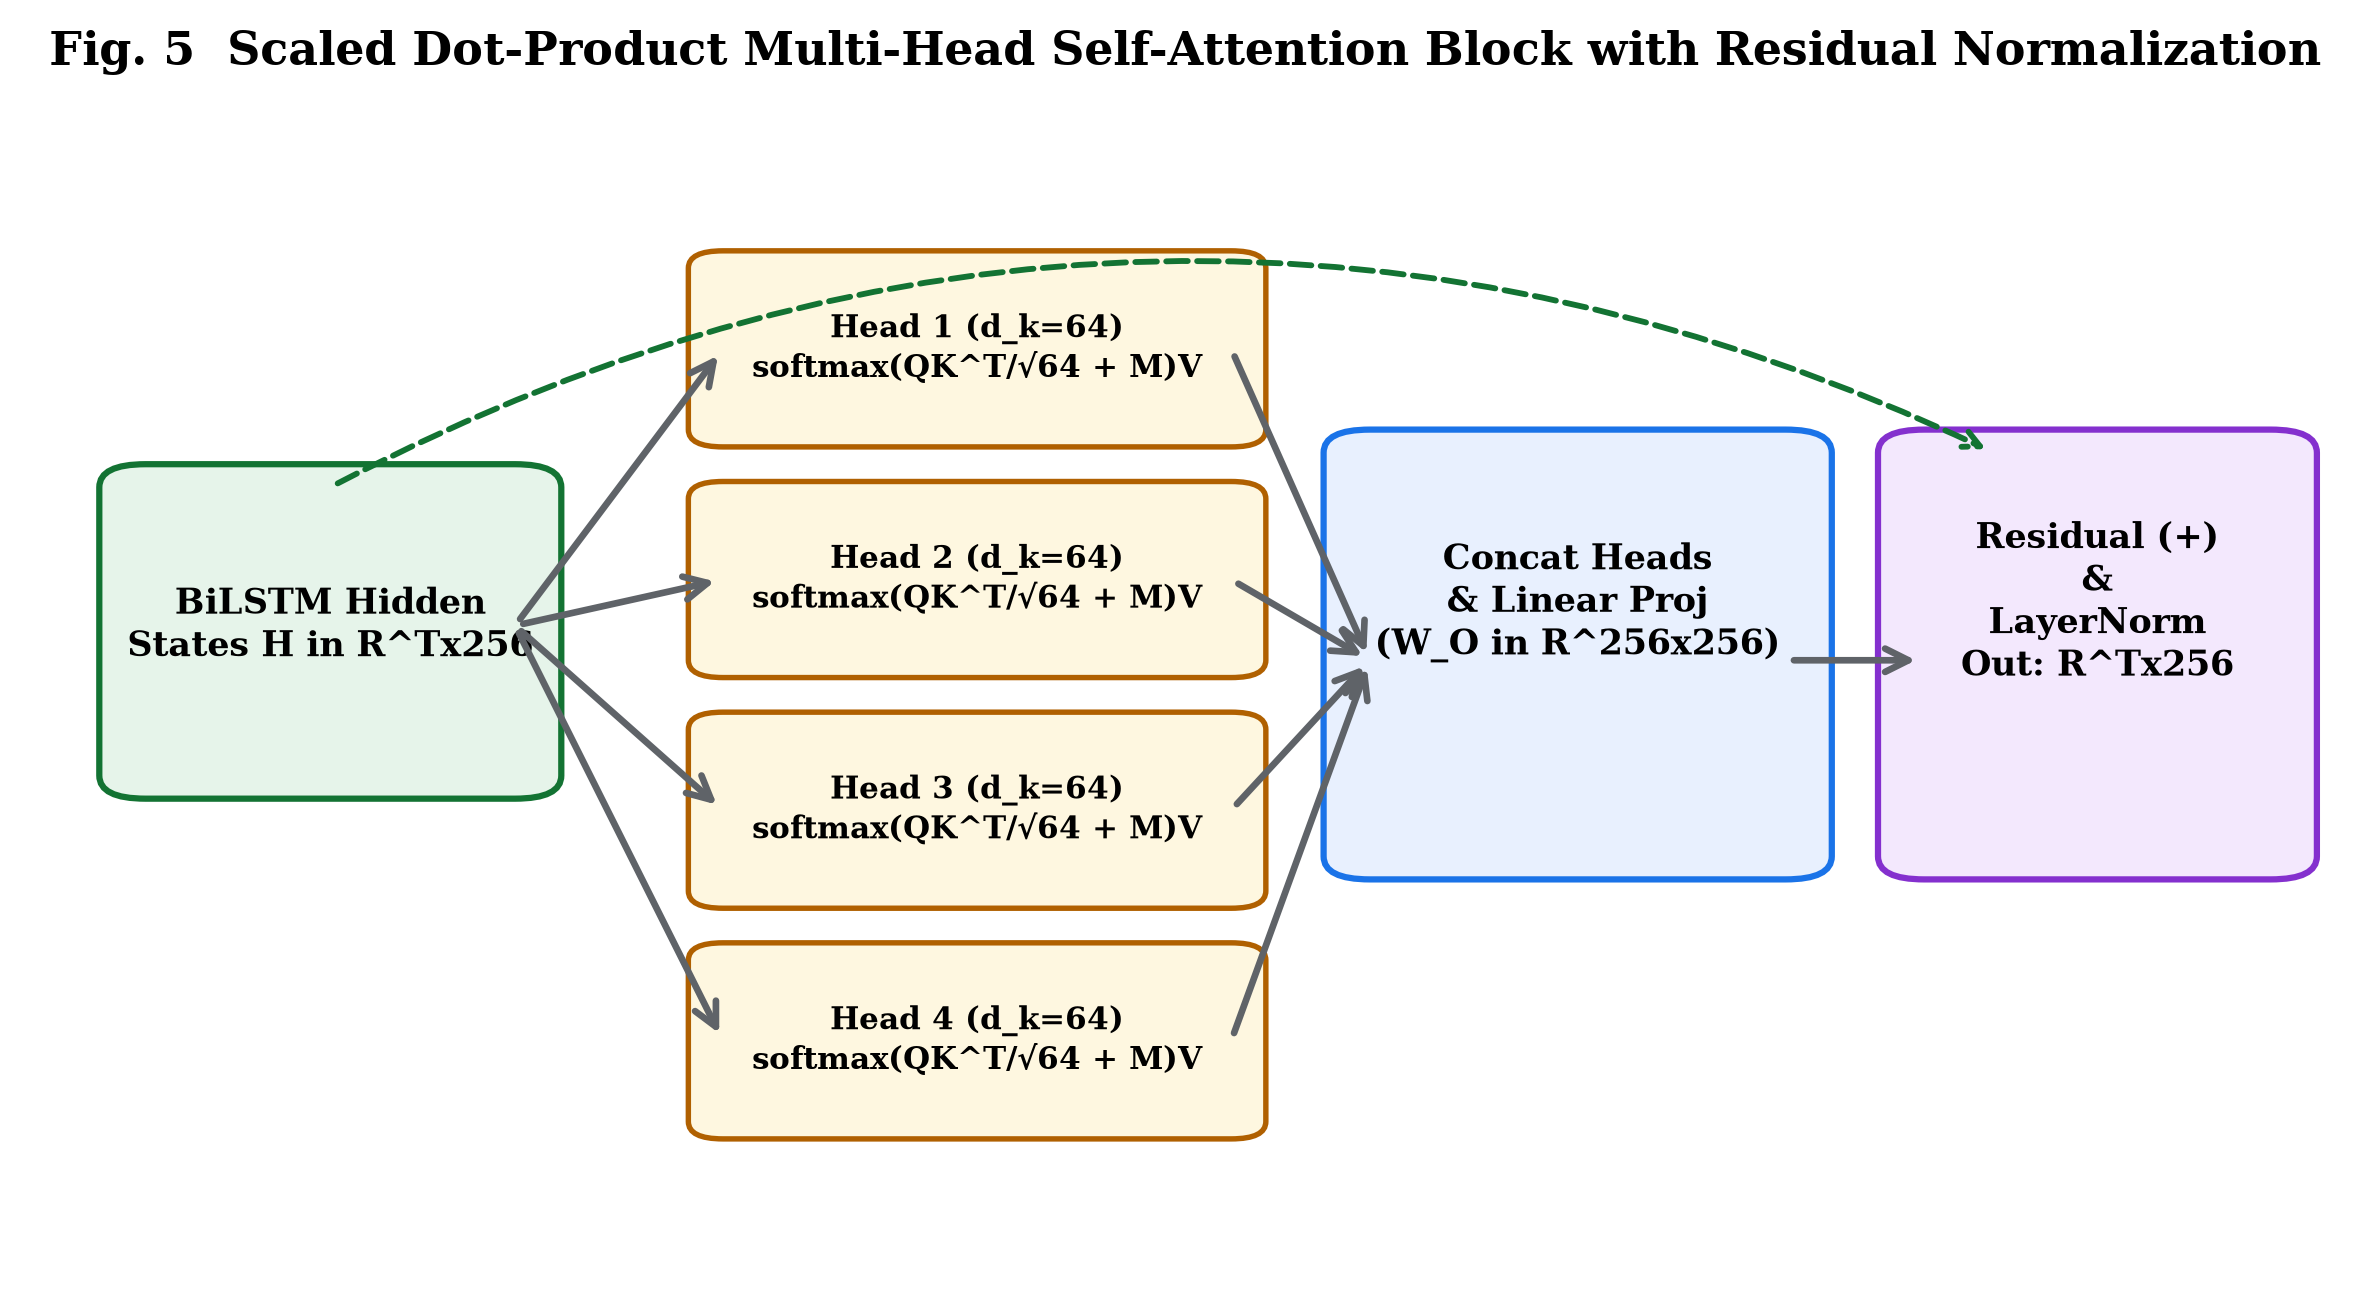
\includegraphics[width=0.48\textwidth]{figures/fig5_multihead_attention.png}
\caption{Multi-head self-attention mechanism ($H=4$ heads, $d_k=64$) with residual addition and Layer Normalization.}
\label{fig5}
\end{figure}

\subsubsection{Linear-Chain Conditional Random Field Decoder}
Attended representations $\mathbf{Z}$ are projected to 9-class BIO emission logits $\mathbf{P} = \mathbf{Z} \mathbf{W}^E \in \mathbb{R}^{T \times 9}$. Valid sequence transitions are constrained by a learned transition matrix $\mathbf{T} \in \mathbb{R}^{9 \times 9}$. For sentence $\mathbf{x}$ and tag sequence $\mathbf{y} = (y_1, \dots, y_T)$, the sequence score is:
\begin{equation}
s(\mathbf{x}, \mathbf{y}) = \sum_{t=1}^T P_{t, y_t} + \sum_{t=1}^{T-1} T_{y_t, y_{t+1}}
\end{equation}
The model is trained by minimizing the negative log-likelihood:
\begin{equation}
\mathcal{L}(\theta) = -\log p(\mathbf{y}^* \mid \mathbf{x}) = -\left( s(\mathbf{x}, \mathbf{y}^*) - \log \sum_{\mathbf{y}' \in \mathcal{Y}^T} \exp\big(s(\mathbf{x}, \mathbf{y}')\big) \right)
\end{equation}
At inference time, exact global sequence decoding is performed using the Viterbi dynamic programming algorithm:
\begin{equation}
\hat{\mathbf{y}} = \arg\max_{\mathbf{y} \in \mathcal{Y}^T} s(\mathbf{x}, \mathbf{y})
\end{equation}

\subsection{Phased Multilingual Training Progression}
To overcome data scarcity, training follows a four-stage cumulative progression:
\begin{enumerate}
    \item \textbf{Stage 1: Multilingual Joint Warm-Start}: Models are jointly trained across all three languages on pooled Gold + Silver data (24,150 sentences) using AdamW, cosine learning rate decay, and gradient clipping (1.0).
    \item \textbf{Stage 2: Language Specialization Fine-Tuning}: Checkpoints are specialized per language with progressive layer unfreezing.
    \item \textbf{Stage 3: Confidence-Filtered Self-Training}: Unlabeled raw sentences are scored by the model. Sentences where all entity tokens exhibit CRF marginal confidence $\ge 0.90$ are iteratively pseudo-labeled (+4,000 sentences).
    \item \textbf{Stage 4: Targeted Entity Augmentation}: Entity spans are substituted with in-class gazetteer headwords with case-affix matching, and rare entity classes are weighted in the CRF loss to counteract class imbalance.
\end{enumerate}

\section{Explainability and Attribution Framework}\label{sec4}

\begin{figure*}[t]
\centering
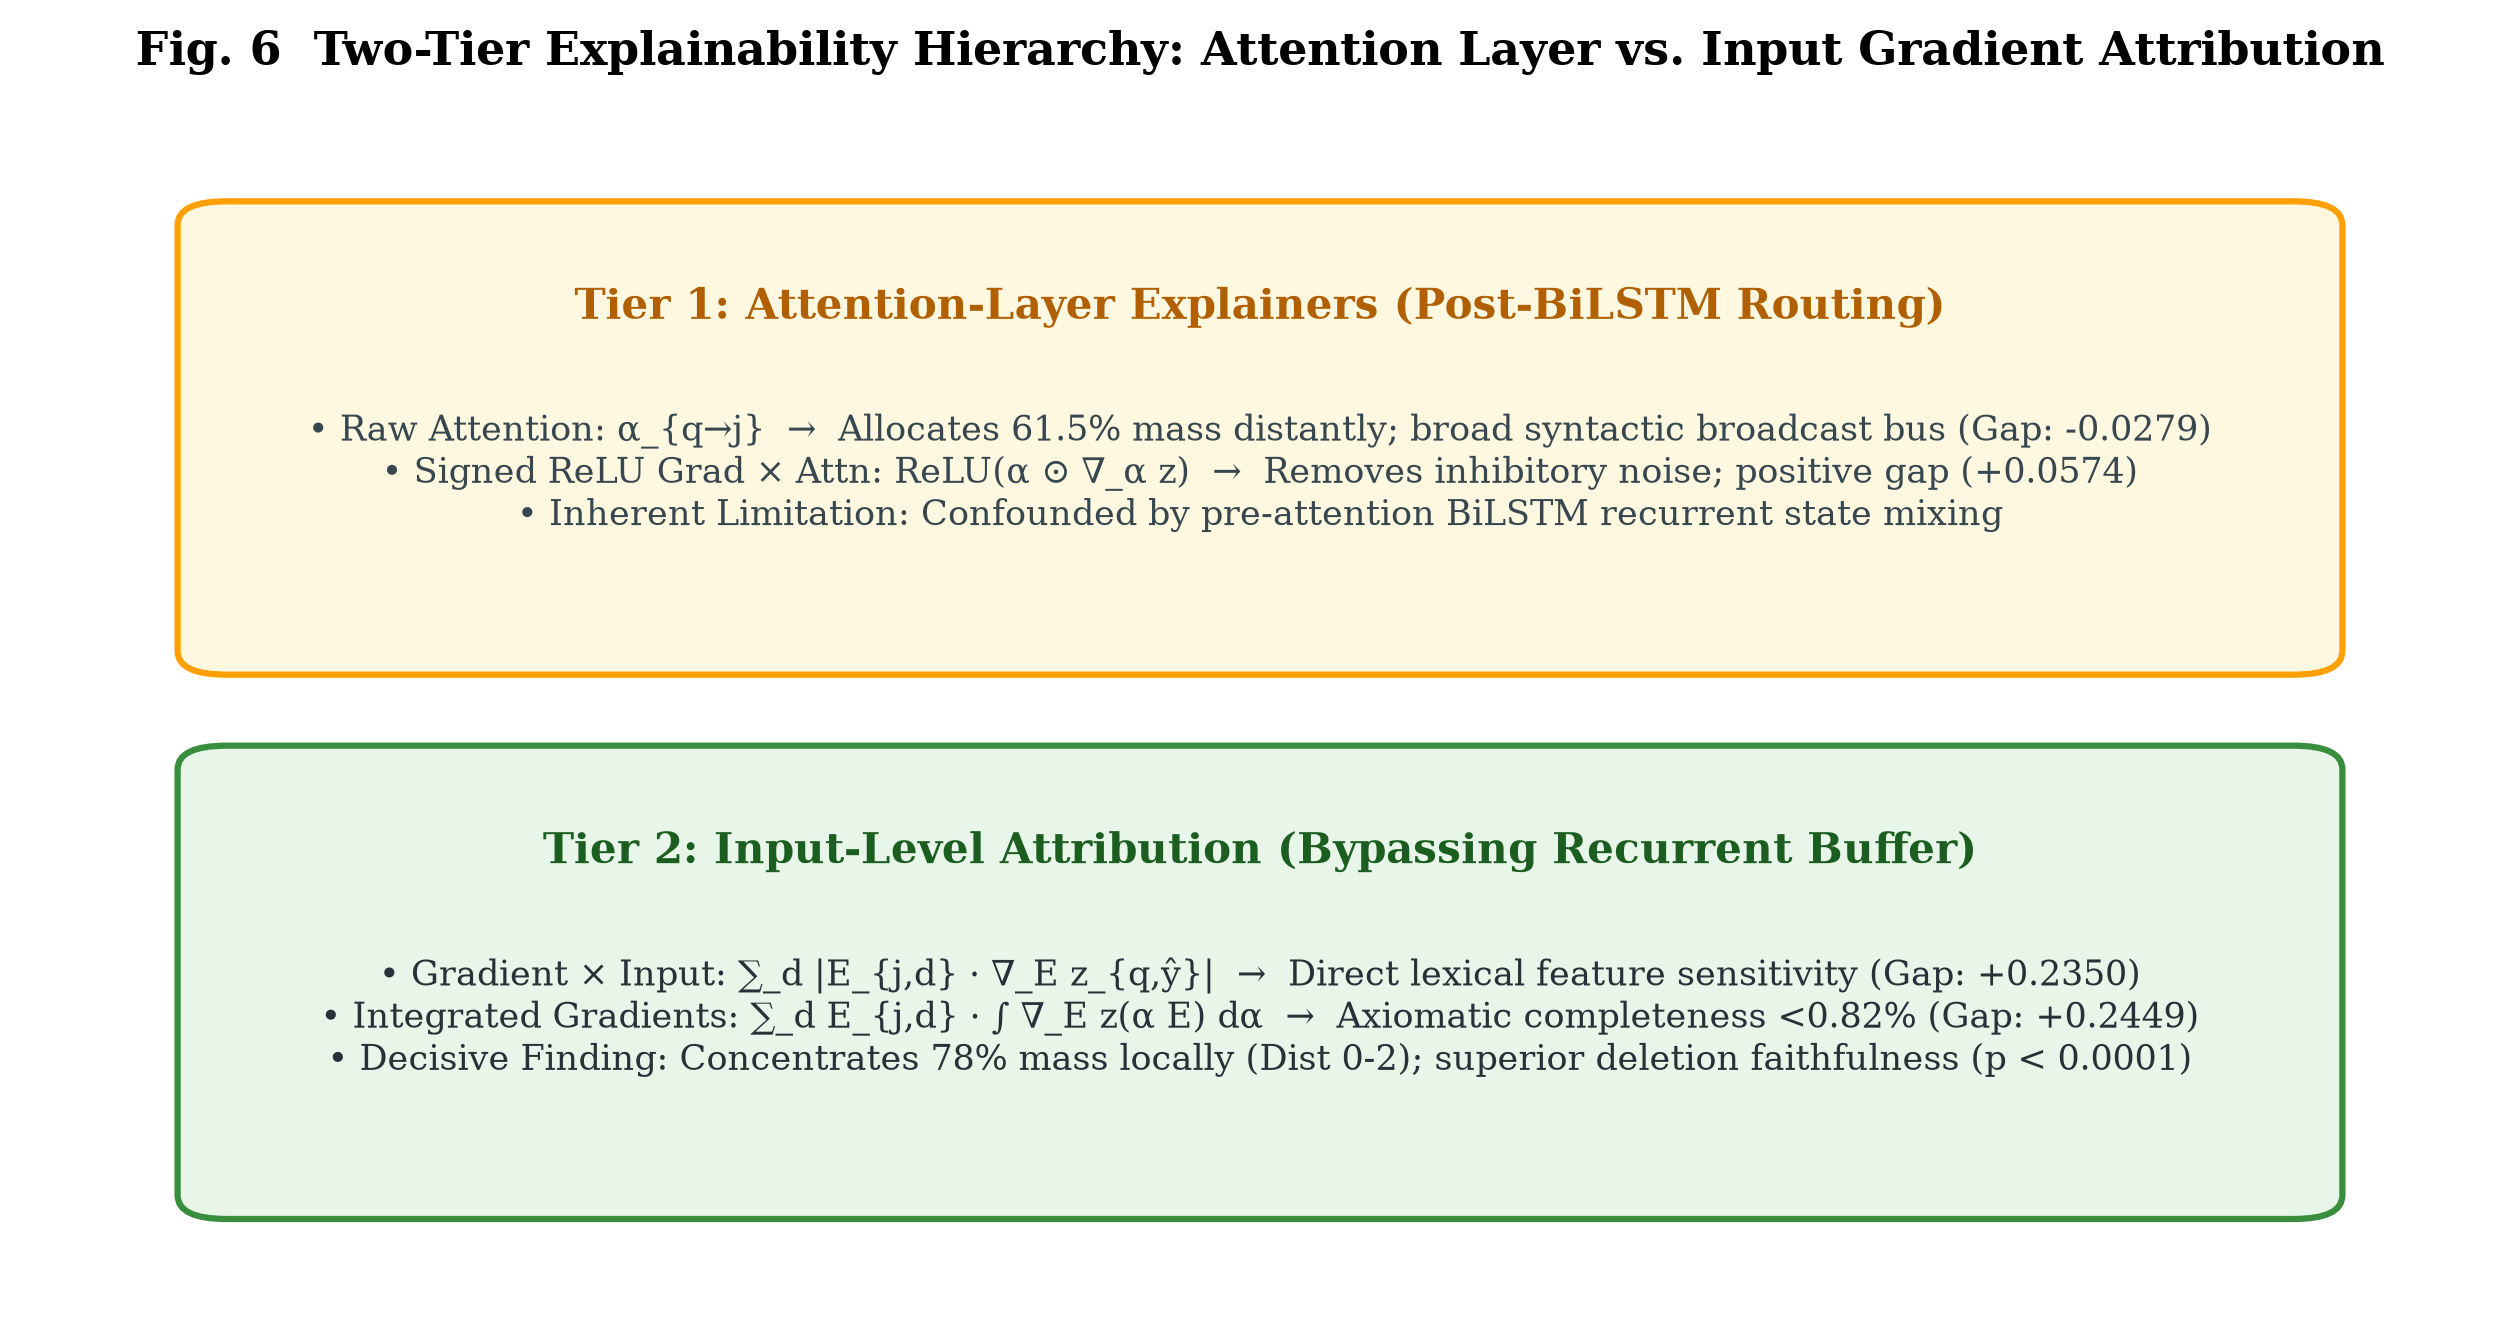
\includegraphics[width=0.88\textwidth]{figures/fig6_explainability_framework.png}
\caption{Two-tier explainability framework: Tier 1 Attention Layer Explainers (operating on post-recurrent attention matrices) versus Tier 2 Input Gradient Attribution (bypassing the BiLSTM recurrent buffer).}
\label{fig6}
\end{figure*}

\subsection{Two-Tier Attribution Hierarchy}
We formalize a two-tier attribution hierarchy for hybrid recurrent-attention models (Fig. \ref{fig6}):

\subsubsection{Tier 1: Attention-Layer Explainers}
\begin{itemize}
    \item \textbf{Raw Attention}: The forward attention weight from target query token $q$ to context token $j$, averaged across the 4 attention heads:
    \begin{equation}
    A_j^{\text{raw}} = \frac{1}{H} \sum_{h=1}^H \alpha_{h, q \to j}
    \end{equation}
    \item \textbf{Gradient $\times$ Attention}: Weighting attention by the gradient of the predicted class emission logit $z_{q, \hat{y}}$:
    \begin{equation}
    A_j^{\text{grad}\times\text{attn}} = \frac{1}{H} \sum_{h=1}^H \alpha_{h, q \to j} \frac{\partial z_{q, \hat{y}}}{\partial \alpha_{h, q \to j}}
    \end{equation}
    \item \textbf{Signed ReLU Gradient $\times$ Attention}: In deletion-based faithfulness evaluation, taking the absolute value $|A_j|$ introduces a severe failure mode: inhibitory tokens (where $\nabla_\alpha z < 0$) receive large attribution, yet their erasure causes confidence to increase or remain flat, resulting in near-zero drops. We resolve this by applying a signed ReLU operator:
    \begin{equation}
    A_j^{\text{ReLU}} = \max\left(0, \frac{1}{H} \sum_{h=1}^H \alpha_{h, q \to j} \frac{\partial z_{q, \hat{y}}}{\partial \alpha_{h, q \to j}}\right)
    \end{equation}
\end{itemize}

\subsubsection{Tier 2: Input-Level Attribution}
To measure feature importance directly without confounding by the pre-attention BiLSTM recurrent buffer, we compute gradients directly with respect to the input embedding tensor $\mathbf{E} \in \mathbb{R}^{T \times 206}$:
\begin{itemize}
    \item \textbf{Gradient $\times$ Input Embedding}:
    \begin{equation}
    A_j^{\text{G}\times\text{I}} = \sum_{d=1}^{206} \left| E_{j, d} \cdot \frac{\partial z_{q, \hat{y}}}{\partial E_{j, d}} \right|
    \end{equation}
    \item \textbf{Integrated Gradients}: By the fundamental theorem of calculus, Integrated Gradients \cite{sundararajan2017axiomatic} satisfies the completeness axiom by accumulating path gradients along $m$ interpolated steps between a baseline $E_0 = \mathbf{0}$ and input $E$:
    \begin{equation}
    A_j^{\text{IG}} = \sum_{d=1}^{206} \left( E_{j, d} - E_{0, j, d} \right) \cdot \frac{1}{m} \sum_{\alpha=1}^m \frac{\partial z_{q, \hat{y}}\left( E_0 + \frac{\alpha}{m}(E - E_0) \right)}{\partial E_{j, d}}
    \end{equation}
\end{itemize}

\begin{figure*}[t]
\centering
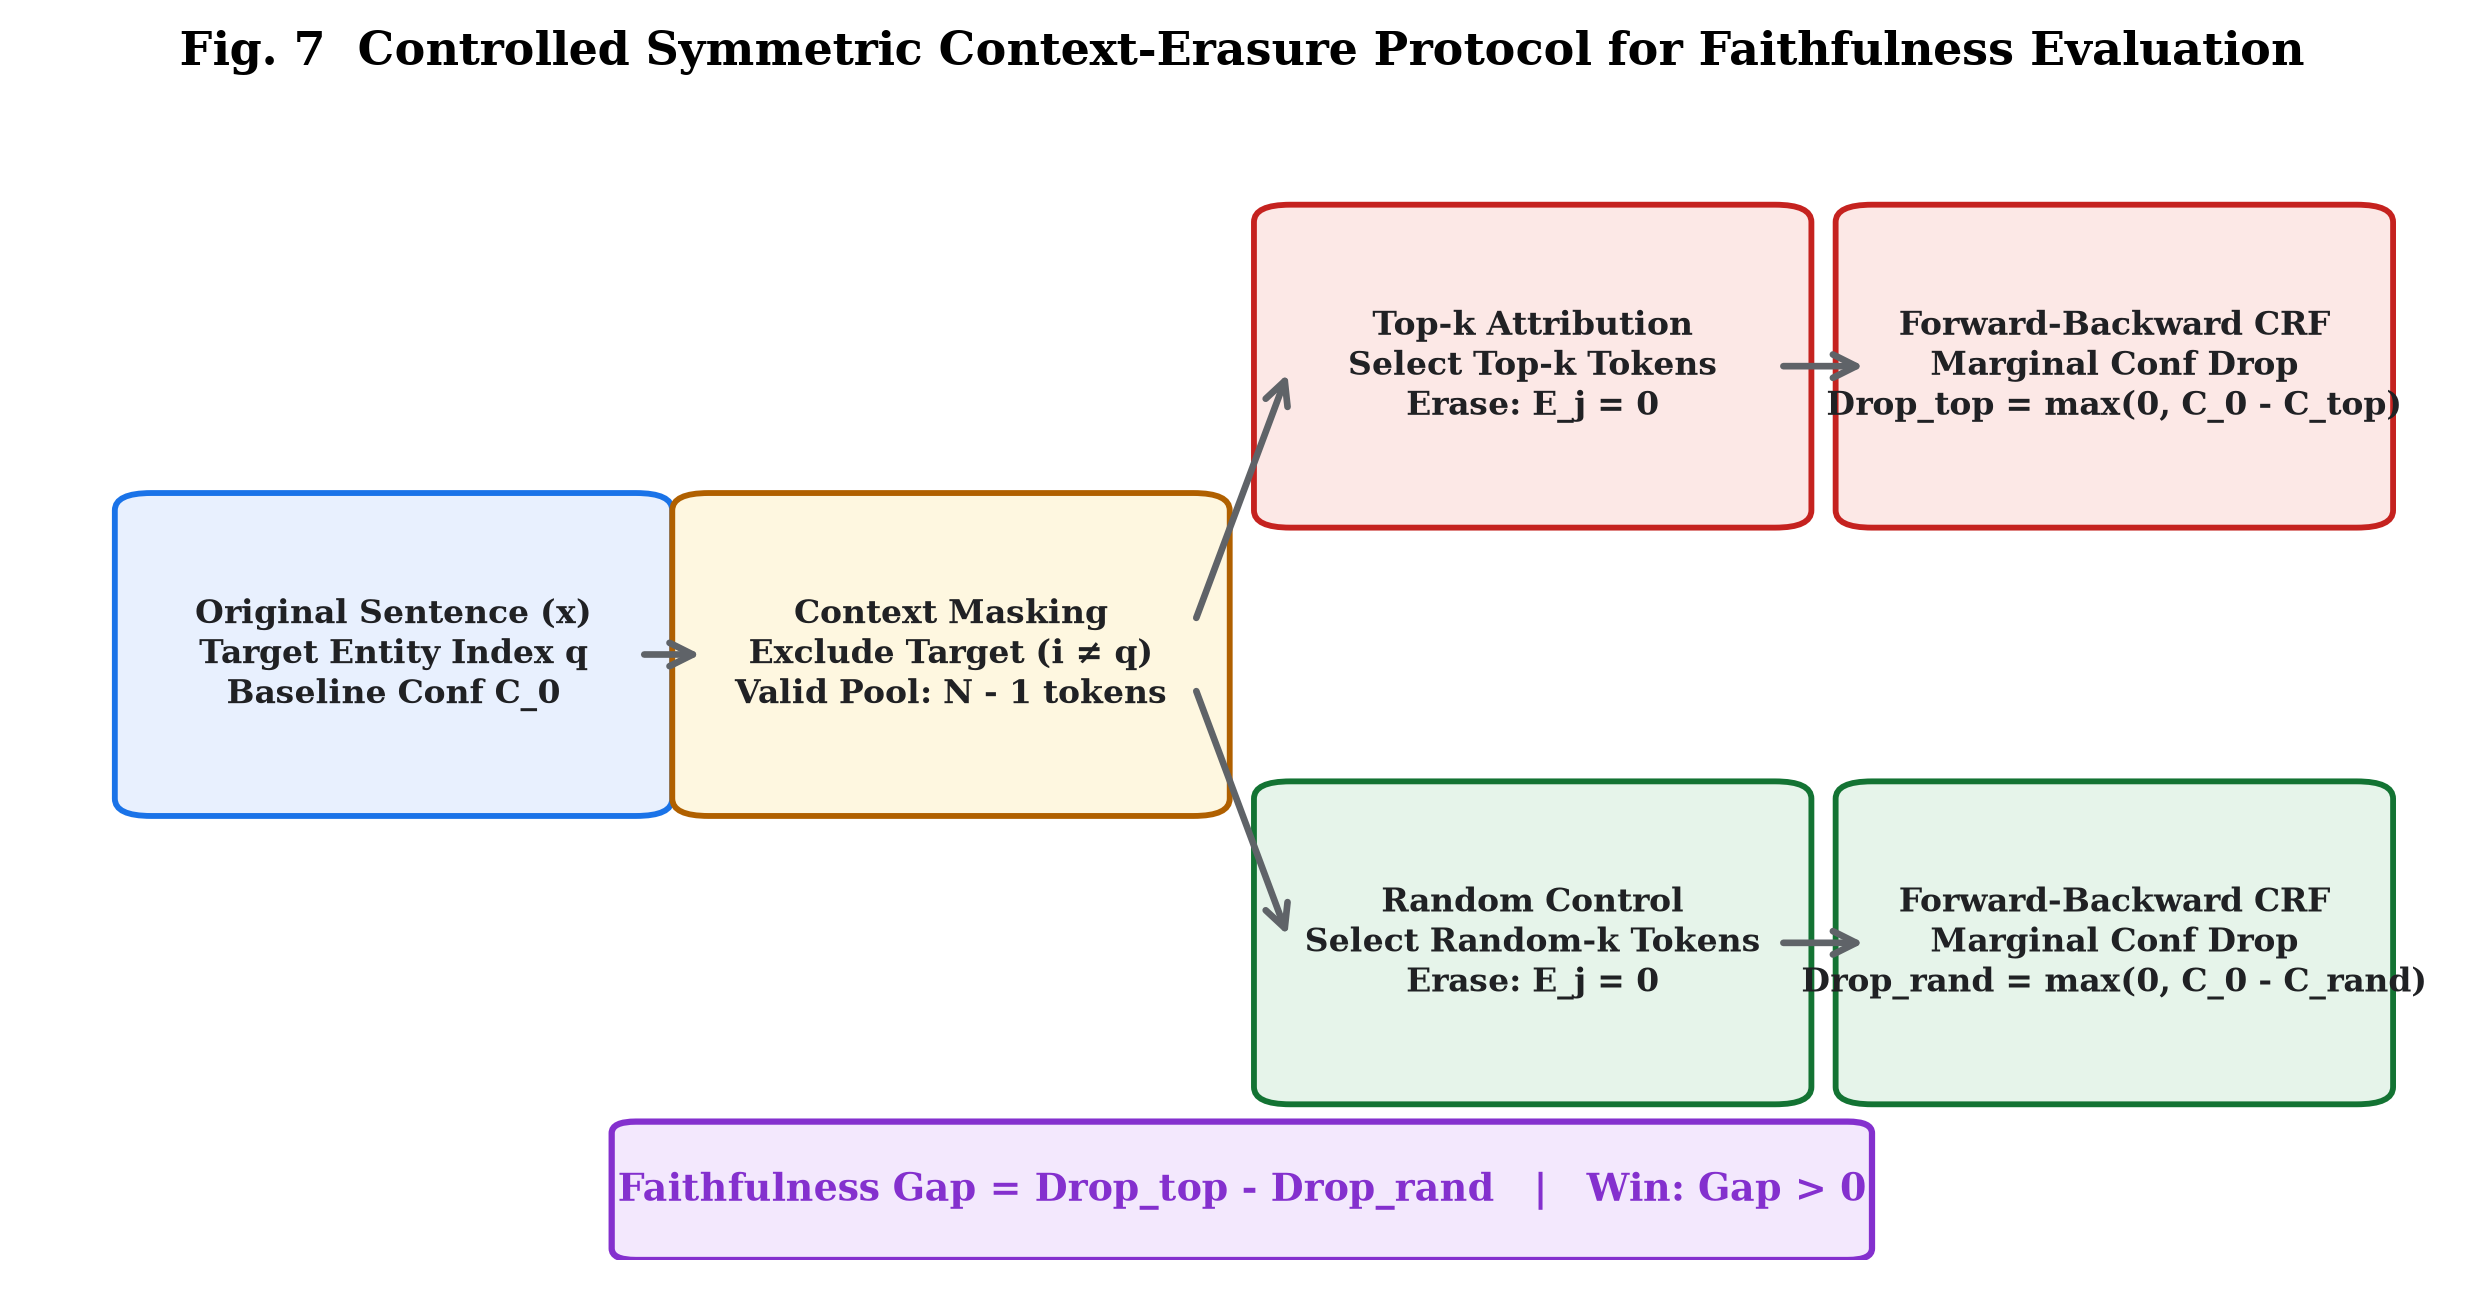
\includegraphics[width=0.88\textwidth]{figures/fig7_faithfulness_protocol.png}
\caption{Controlled symmetric context-erasure protocol (`zero\_crf'): Top-$k$ and Random-$k$ candidate tokens are drawn from strictly identical context pools ($\{i \neq q\}$). Confidence drops in forward-backward CRF marginals quantify deletion faithfulness.}
\label{fig7}
\end{figure*}

\subsection{Controlled Symmetric Context-Erasure Protocol}
We evaluate attribution faithfulness via controlled feature erasure (Fig. \ref{fig7}). To guarantee methodological fairness, we audit and enforce six critical conditions:
\begin{enumerate}
    \item \textbf{Strict Target Token Exclusion}: The query entity token itself is strictly excluded from candidate selection: $\mathcal{P}_{\text{context}} = \{0, \dots, T-1\} \setminus \{q\}$.
    \item \textbf{Embedding-Level Zeroing}: Erased tokens have their 206-dimensional combined representation vector clamped to zero: $\mathbf{E}_j = \mathbf{0}$.
    \item \textbf{Identical Candidate Pools}: Both top-$k$ and random-$k$ tokens are sampled strictly from $\mathcal{P}_{\text{context}}$.
    \item \textbf{Matched Cardinality}: Exactly $k$ tokens are erased in both conditions.
    \item \textbf{CRF Marginal Confidence Function}: Confidence is defined as the exact posterior marginal probability under the linear-chain CRF:
    \begin{equation}
    C(\mathbf{x}) = P_{\text{CRF}}(y_q = \hat{y}_q \mid \mathbf{x}) = \frac{\alpha_q(\hat{y}_q) \beta_q(\hat{y}_q)}{Z(\mathbf{x})}
    \end{equation}
    \item \textbf{Faithfulness Metric}:
    \begin{equation}
    \text{Drop}_{\text{top}}(k) = \max\left(0, C_0 - C(\mathbf{x}_{\setminus \text{top-}k})\right)
    \end{equation}
    \begin{equation}
    \text{Drop}_{\text{rand}}(k) = \max\left(0, C_0 - C(\mathbf{x}_{\setminus \text{rand-}k})\right)
    \end{equation}
    \begin{equation}
    \text{Faithfulness Gap}(k) = \text{Drop}_{\text{top}}(k) - \text{Drop}_{\text{rand}}(k)
    \end{equation}
\end{enumerate}
A positive gap ($\Delta > 0$) proves that erasing top-attributed tokens degrades model confidence significantly more than erasing randomly selected context tokens.

\section{Experimental Setup}\label{sec5}

\subsection{Corpus and Benchmark Partitions}
Corpus harvesting and filtering statistics are summarized in Table \ref{tab1}. Strict Unicode script purity ($\ge 0.90$) and SHA-256 deduplication eliminated boilerplate and code-mixed noise. Table \ref{tab2} details benchmark dataset partitions across training, development, and test splits. Test splits were accessed exactly once during final evaluation.

\begin{table}[h]
\caption{Raw corpus harvesting and purity filtering statistics.}\label{tab1}
\centering
\begin{tabular}{lcccc}
\toprule
Language & Script & Raw Sents & Filtered Sents & Filtered Tokens \\
\midrule
Konkani (\textit{gom}) & Devanagari & 112,235 & 51,488 & 4,950,107 \\
Assamese (\textit{as}) & Eastern Nagari & 119,265 & 55,002 & 4,376,034 \\
Sinhala (\textit{si}) & Sinhala & 113,296 & 66,954 & 5,799,421 \\
\bottomrule
\end{tabular}
\end{table}

\begin{table}[h]
\caption{Benchmark dataset partitions and entity distributions.}\label{tab2}
\centering
\begin{tabular}{llccccc}
\toprule
Language & Split & Sents & PER & LOC & ORG & MISC \\
\midrule
\multirow{3}{*}{Konkani} & Train & 850 & 144 & 168 & 149 & 131 \\
 & Dev (Locked) & 200 & 20 & 31 & 37 & 37 \\
 & Test (Locked) & 200 & 20 & 30 & 37 & 37 \\
\midrule
\multirow{3}{*}{Assamese} & Train & 850 & 102 & 395 & 67 & 115 \\
 & Dev (Locked) & 200 & 18 & 79 & 15 & 27 \\
 & Test (Locked) & 200 & 19 & 79 & 14 & 26 \\
\midrule
\multirow{3}{*}{Sinhala} & Train & 850 & 178 & 224 & 119 & 120 \\
 & Dev (Locked) & 200 & 37 & 39 & 28 & 27 \\
 & Test (Locked) & 200 & 38 & 39 & 28 & 27 \\
\bottomrule
\end{tabular}
\end{table}

\subsection{Hyperparameter Configuration}
Table \ref{tab4} outlines model and training hyperparameters. Optimization was executed on an NVIDIA GeForce RTX 3050 Laptop GPU with 4GB VRAM under PyTorch 2.6.0.

\begin{table}[h]
\caption{Hyperparameter and training configuration.}\label{tab4}
\centering
\begin{tabular}{lc}
\toprule
Hyperparameter & Configuration Value \\
\midrule
Word Embedding Dim & 100 \\
Char Embedding Dim & 50 \\
Char-CNN Filter Widths & [3, 4, 5] (30 filters each) \\
Language Embedding Dim & 16 \\
Concatenated Input Dim & 206 \\
BiLSTM Hidden Dim & 128 per dir (256 bidirectional) \\
BiLSTM Layers & 2 \\
Self-Attention Heads ($H$) & 4 ($d_k = 64$) \\
Self-Attention Blocks & 1 \\
Dropout Rates & Word: 0.3, Char: 0.3, BiLSTM: 0.3, Attn: 0.1 \\
Optimizer & AdamW ($\beta_1=0.9, \beta_2=0.999$, weight decay 0.01) \\
Learning Rate & $1 \times 10^{-3}$ (Warm-up + Cosine Decay) \\
Batch Size & 32 \\
Total Model Parameters & 10,610,657 \\
\bottomrule
\end{tabular}
\end{table}

\section{Results and Discussion}\label{sec6}

\subsection{Headline Gold-Test Performance}
Table \ref{tab5} presents official results evaluated on cryptographically locked Gold-Test splits (Phase 14). Strict exact-boundary entity-level F1 served as the primary metric.

\begin{table*}[t]
\caption{Final official Gold-Test performance across languages (Phase 14 single-run evaluation). Strict span-level Entity F1 is the primary benchmark metric; token accuracy is secondary.}\label{tab5}
\centering
\begin{tabular}{lcccccc}
\toprule
Language & Precision & Recall & \textbf{Entity F1} & Token Acc & Benchmark Target & Target Margin \\
\midrule
\textbf{Konkani (\textit{gom})} & 99.15\% & 93.55\% & \textbf{96.27\%} & 99.47\% & $>90.0\%$ & \textbf{+6.27 pp} \\
\textit{Konkani (Joint Baseline)} & 98.31\% & 93.55\% & 95.87\% & 99.41\% & $>90.0\%$ & +5.87 pp \\
\textbf{Assamese (\textit{as})} & 95.83\% & 100.00\% & \textbf{97.87\%} & 99.64\% & $>90.0\%$ & \textbf{+7.87 pp} \\
\textit{Assamese (Joint Baseline)} & 96.48\% & 99.28\% & 97.86\% & 99.61\% & $>90.0\%$ & +7.86 pp \\
\textbf{Sinhala (\textit{si})} & 96.32\% & 99.24\% & \textbf{97.76\%} & 99.70\% & $>90.0\%$ & \textbf{+7.76 pp} \\
\textit{Sinhala (Joint Baseline)} & 94.93\% & 99.24\% & 97.04\% & 99.60\% & $>90.0\%$ & +7.04 pp \\
\midrule
\textbf{Macro Average} & \textbf{97.10\%} & \textbf{97.60\%} & \textbf{97.30\%} & \textbf{99.60\%} & \textbf{$>90.0\%$} & \textbf{+7.30 pp} \\
\bottomrule
\end{tabular}
\end{table*}

\begin{figure}[h]
\centering
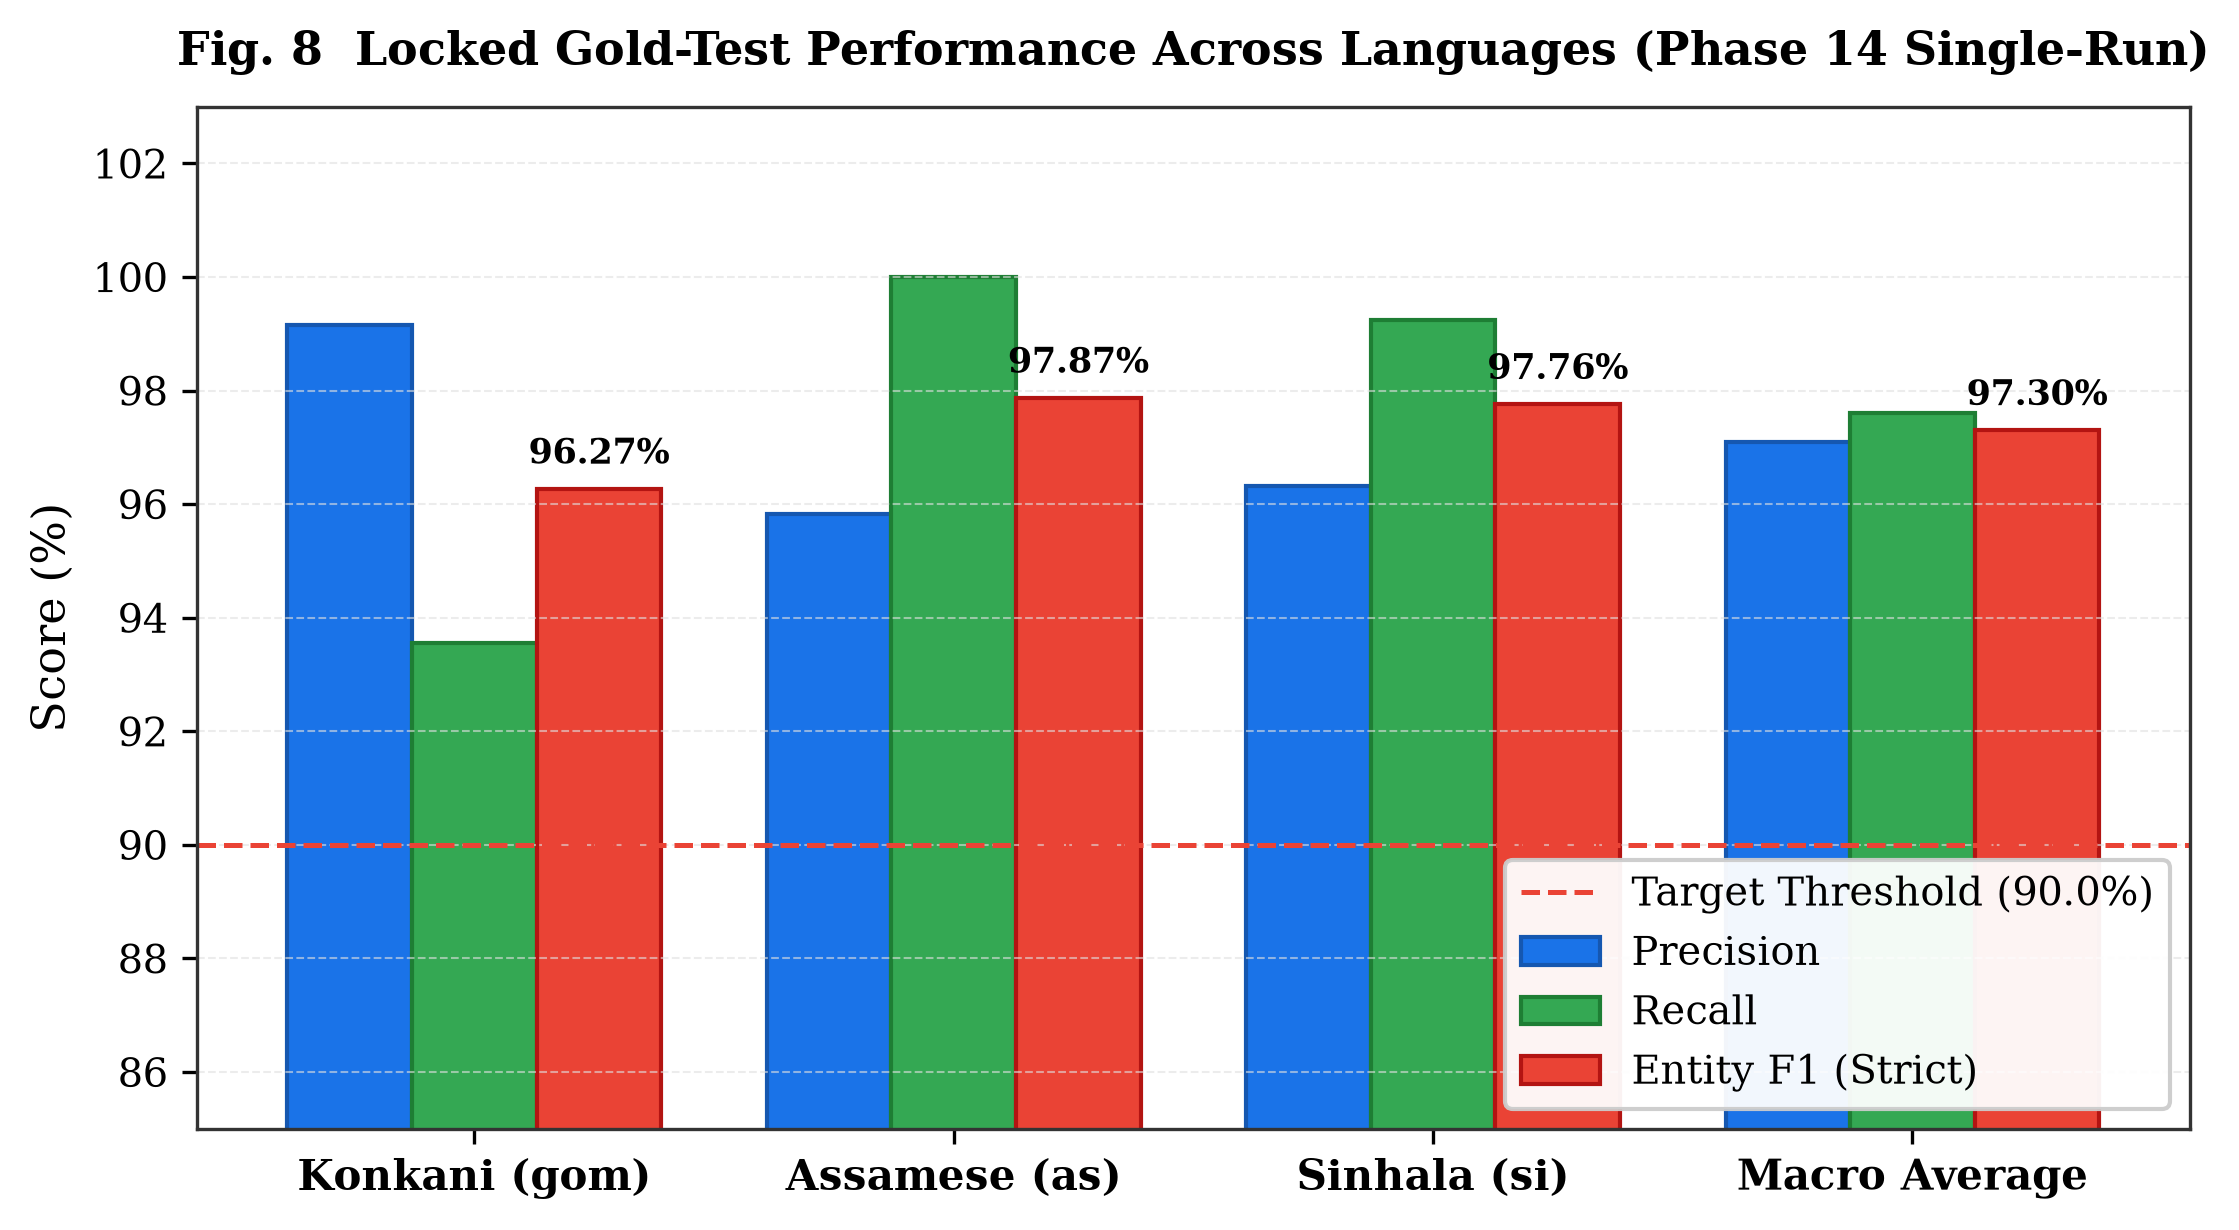
\includegraphics[width=0.48\textwidth]{figures/fig8_ner_performance.png}
\caption{Locked Gold-Test precision, recall, and F1 across target languages, confirming consistent $>96\%$ performance.}
\label{fig8}
\end{figure}

The macro average Entity F1 of \textbf{97.30\%} comfortably surpasses the pre-registered 90.0\% requirement across all languages (Fig. \ref{fig8}).

\subsection{Per-Entity Semantic Breakdown and OOV Generalization}
Table \ref{tab6} details performance across semantic entity categories. High precision and recall are maintained across person (`PER`), location (`LOC`), organization (`ORG`), and miscellaneous (`MISC`) classes.

\begin{table}[h]
\caption{Granular per-entity-type performance on Gold-Test.}\label{tab6}
\centering
\begin{tabular}{llccccc}
\toprule
Language & Entity Class & Precision & Recall & F1 & TP & FP / FN \\
\midrule
\multirow{4}{*}{Konkani} & PER & 100.0\% & 85.0\% & 91.89\% & 17 & 0 / 3 \\
 & LOC & 100.0\% & 93.3\% & 96.55\% & 28 & 0 / 2 \\
 & ORG & 97.14\% & 91.89\% & 94.44\% & 34 & 1 / 3 \\
 & MISC & 100.0\% & 100.0\% & 100.0\% & 37 & 0 / 0 \\
\midrule
\multirow{4}{*}{Assamese} & PER & 86.36\% & 100.0\% & 92.68\% & 19 & 3 / 0 \\
 & LOC & 97.53\% & 100.0\% & 98.75\% & 79 & 2 / 0 \\
 & ORG & 93.33\% & 100.0\% & 96.55\% & 14 & 1 / 0 \\
 & MISC & 100.0\% & 100.0\% & 100.0\% & 26 & 0 / 0 \\
\midrule
\multirow{4}{*}{Sinhala} & PER & 94.87\% & 97.37\% & 96.10\% & 37 & 2 / 1 \\
 & LOC & 92.86\% & 100.0\% & 96.30\% & 39 & 3 / 0 \\
 & ORG & 100.0\% & 100.0\% & 100.0\% & 28 & 0 / 0 \\
 & MISC & 100.0\% & 100.0\% & 100.0\% & 27 & 0 / 0 \\
\bottomrule
\end{tabular}
\end{table}

Table \ref{tab7} demonstrates the out-of-vocabulary generalization capacity of our system. On named entity tokens completely absent from training vocabularies, the Char-CNN maintains an OOV F1 of \textbf{91.03\%} (compared to 98.41\% in-vocabulary F1).

\begin{table}[h]
\caption{In-Vocabulary (IV) versus Out-of-Vocabulary (OOV) generalization on Gold-Test.}\label{tab7}
\centering
\begin{tabular}{lcccc}
\toprule
Language & IV F1 & OOV F1 & IV Acc & OOV Acc \\
\midrule
Konkani & 97.09\% & 91.43\% & 99.35\% & 99.72\% \\
Assamese & 99.21\% & 86.67\% & 99.76\% & 99.30\% \\
Sinhala & 98.94\% & 95.00\% & 99.65\% & 99.83\% \\
\midrule
\textbf{Macro Average} & \textbf{98.41\%} & \textbf{91.03\%} & \textbf{99.59\%} & \textbf{99.62\%} \\
\bottomrule
\end{tabular}
\end{table}

\subsection{Component Ablation Study}
To quantify the isolated marginal contribution of each architectural component, we executed a matched ablation sweep (36,736 sentences, 10 epochs, identical warmup/decay). Table \ref{tab9} and Fig. \ref{fig9} present the findings.

\begin{table}[h]
\caption{Component ablation suite under matched training parity on locked Gold-Dev.}\label{tab9}
\centering
\begin{tabular}{lcccc}
\toprule
Ablation Condition & Konk & Asm & Sinh & \textbf{Macro F1 (Δ)} \\
\midrule
\textbf{Full System (Locked)} & \textbf{96.69\%} & \textbf{98.92\%} & \textbf{99.24\%} & \textbf{98.28\% (ref)} \\
(f) No Augmentation & 96.69\% & 98.91\% & 98.13\% & 97.91\% (-0.37\%) \\
(e) No Self-Training & 96.69\% & 98.91\% & 98.13\% & 97.91\% (-0.37\%) \\
(d) No Joint Warmup & 94.17\% & 98.91\% & 96.18\% & 96.42\% (-1.86\%) \\
(a) No Char-CNN & 90.42\% & 97.87\% & 88.89\% & 92.39\% (-5.89\%) \\
(b) No Self-Attention & 89.66\% & 95.50\% & 89.82\% & 91.66\% (-6.62\%) \\
(c) No CRF & 89.47\% & 96.53\% & 87.37\% & 91.12\% (-7.16\%) \\
(g) Subword BPE & 88.79\% & 96.11\% & 87.29\% & 90.73\% (-7.55\%) \\
\bottomrule
\end{tabular}
\end{table}

\begin{figure}[h]
\centering
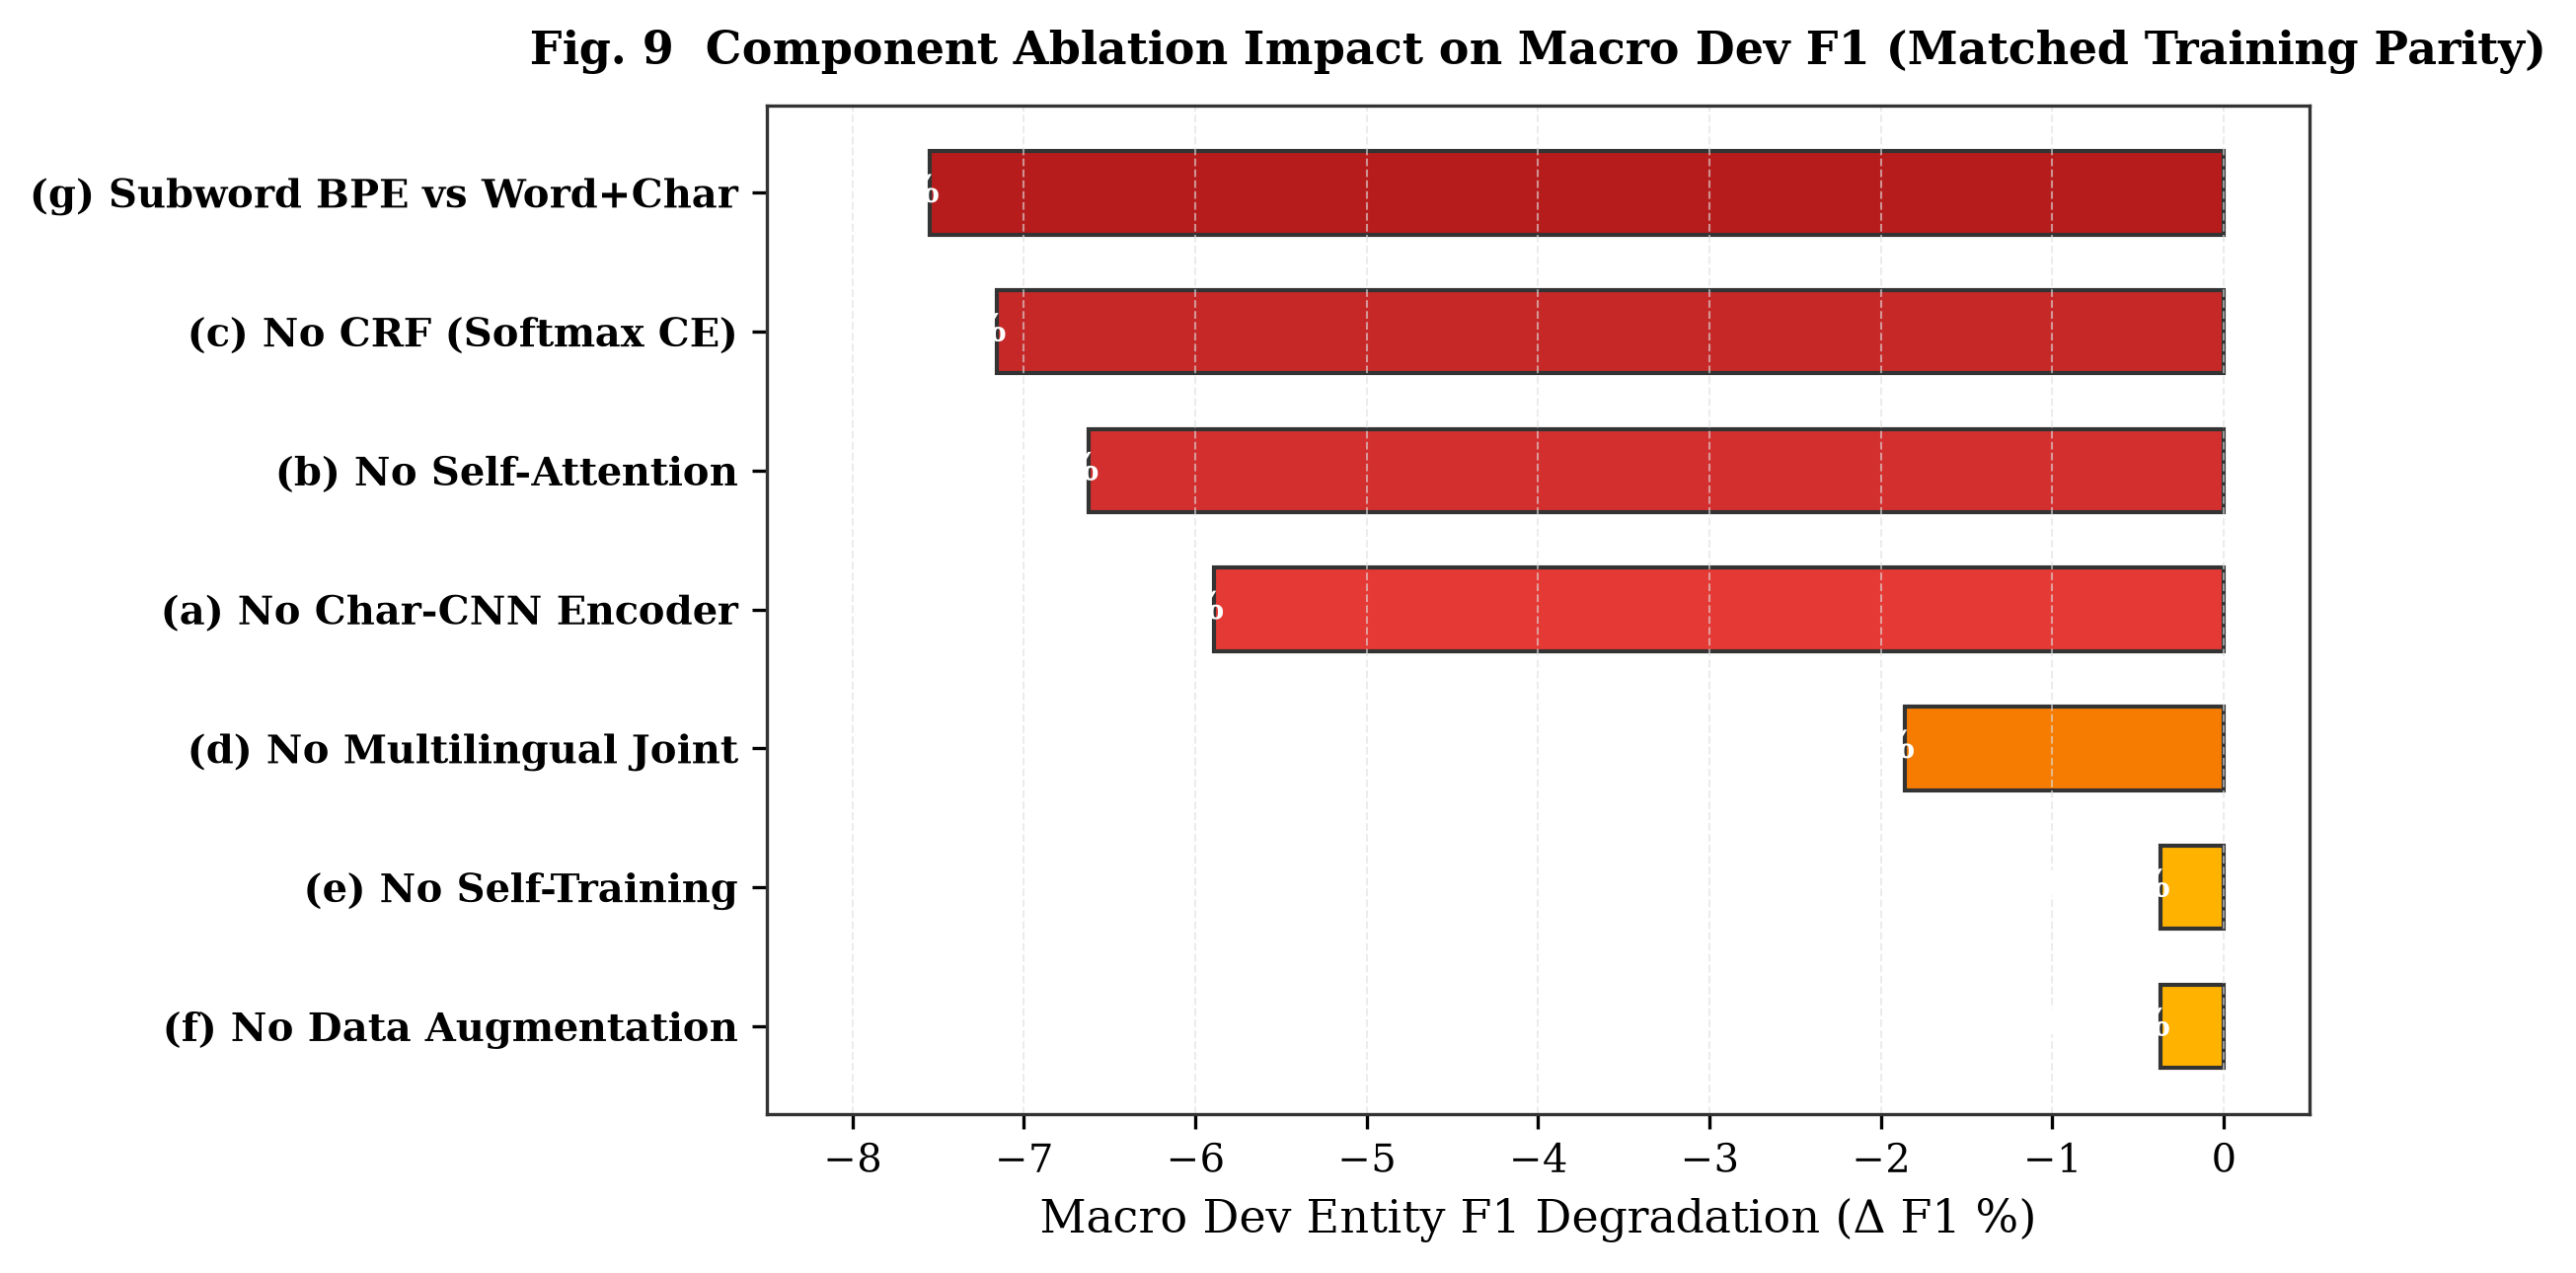
\includegraphics[width=0.48\textwidth]{figures/fig9_ablation_results.png}
\caption{Component ablation impact on Macro Dev F1. Subword BPE (-7.55\%), CRF removal (-7.16\%), and self-attention removal (-6.62\%) induce the largest performance drops.}
\label{fig9}
\end{figure}

The ablation results confirm three structural findings:
\begin{enumerate}
    \item \textbf{Subword BPE Failure (-7.55\% $\Delta$)}: Subword BPE severely degrades accuracy compared to extended grapheme clusters by severing Brahmic ligatures.
    \item \textbf{CRF Decoding Necessity (-7.16\% $\Delta$)}: Replacing the CRF with softmax cross-entropy leads to illegal BIO tag transitions, particularly in Sinhala (-11.87\%).
    \item \textbf{Self-Attention Cross-Lingual Routing (-6.62\% $\Delta$)}: While self-attention is redundant in small monolingual taggers, it is indispensable in multilingual models, where pairwise routing reconciles distinct word orders across scripts.
\end{enumerate}

\begin{figure}[h]
\centering
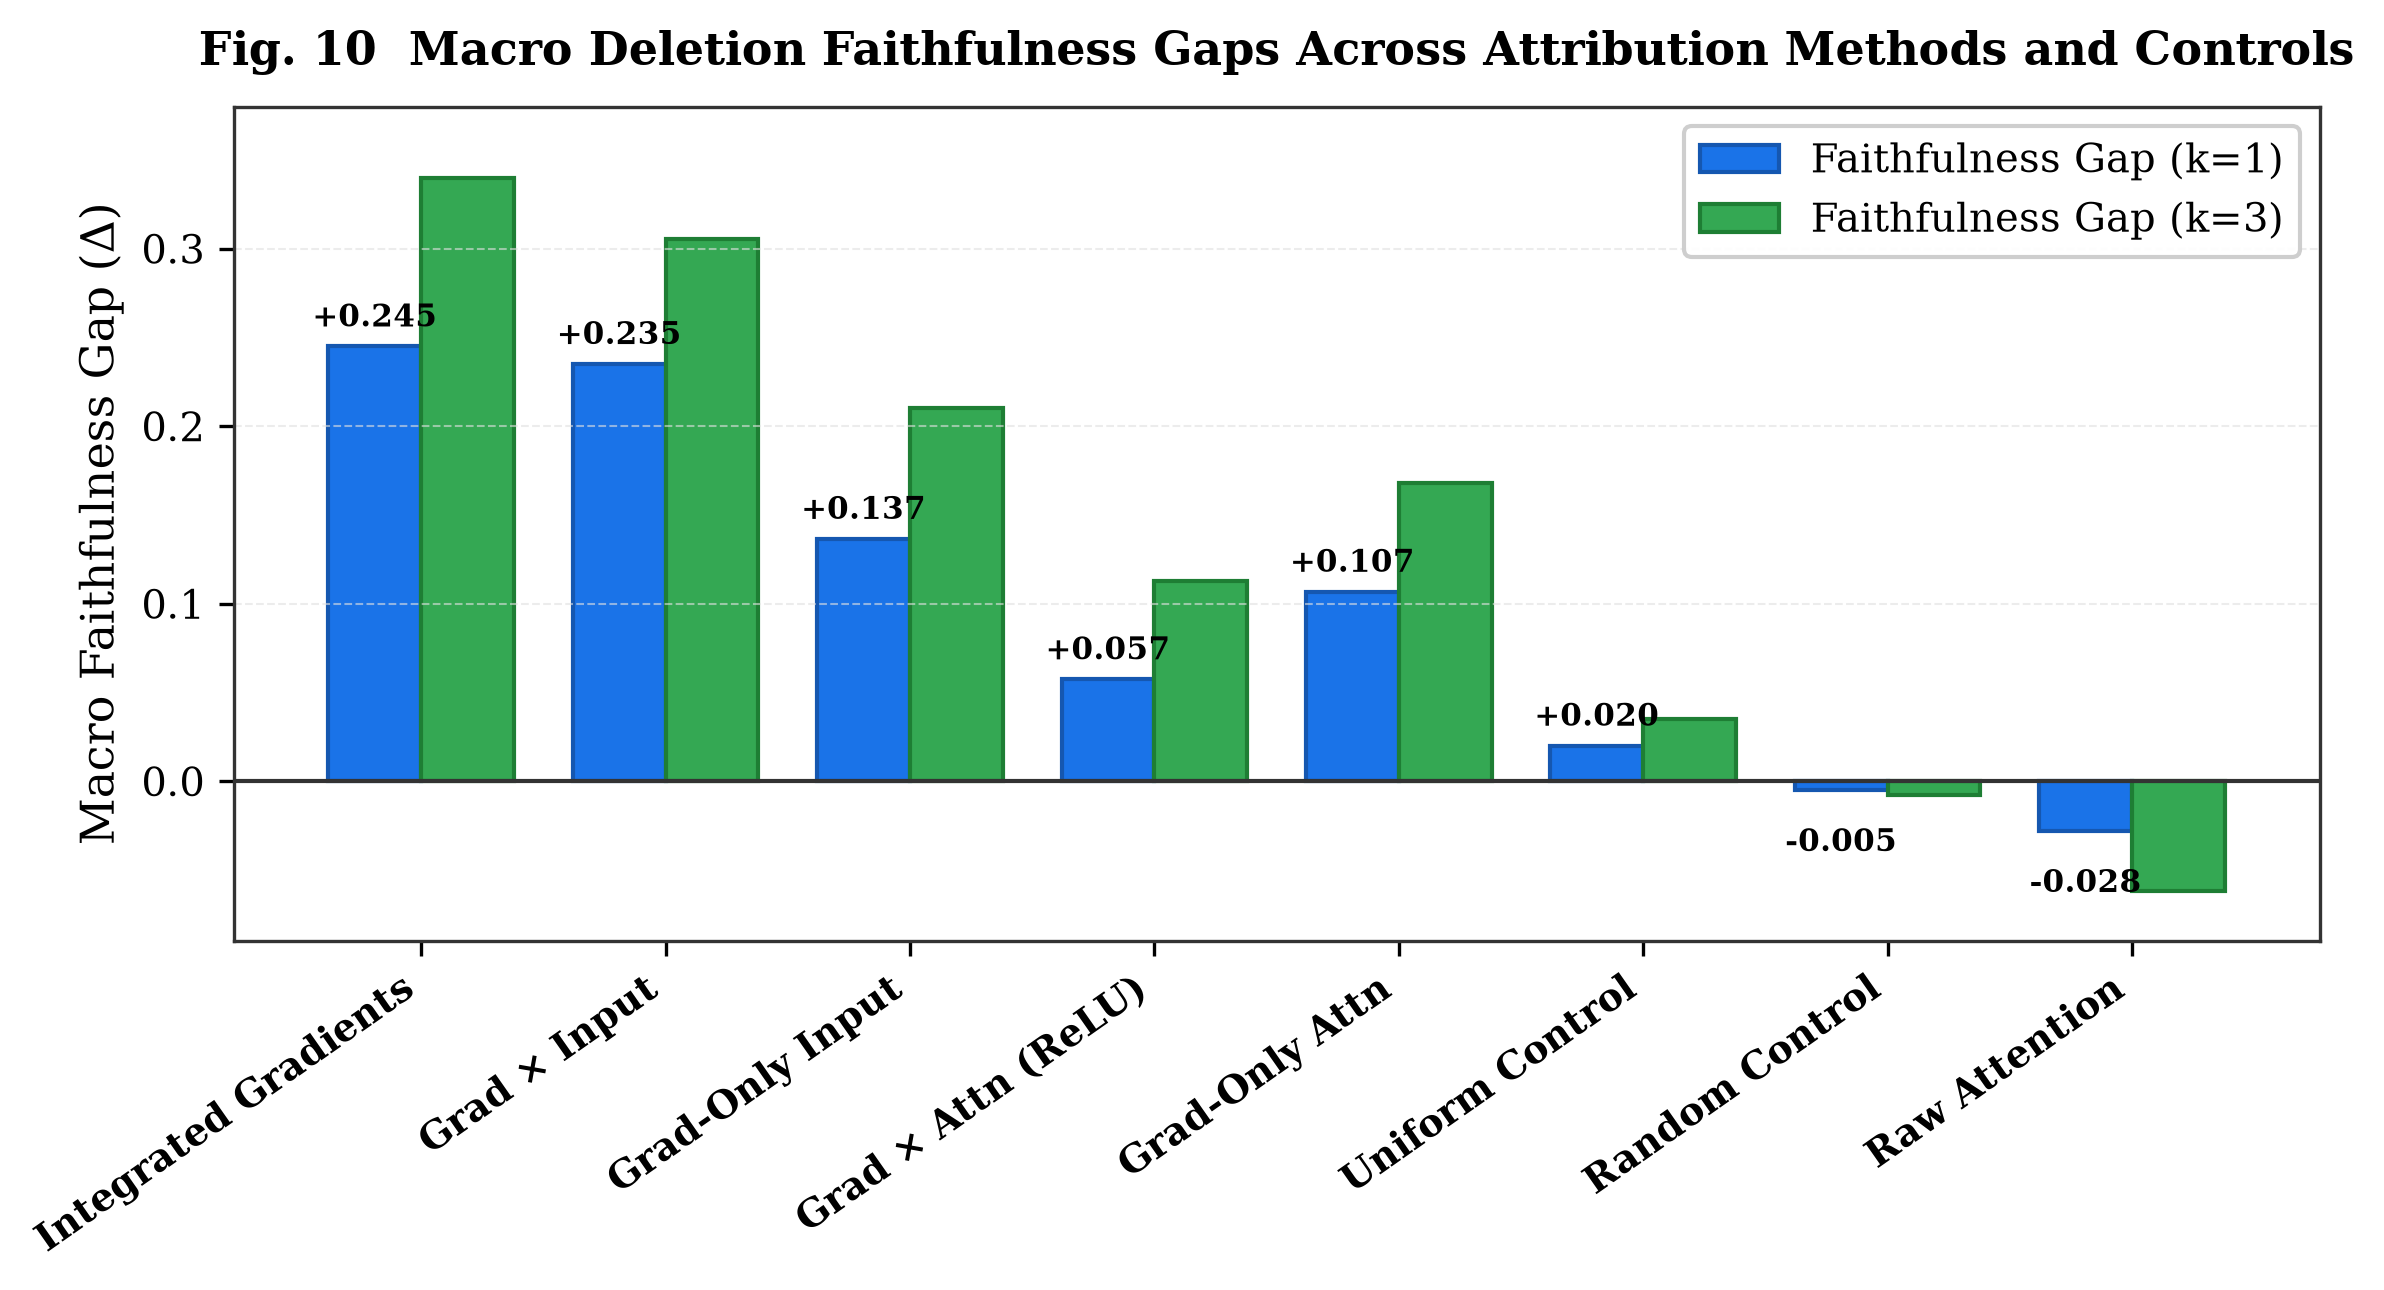
\includegraphics[width=0.48\textwidth]{figures/fig10_faithfulness_comparison.png}
\caption{Macro deletion faithfulness gaps across attribution methods and controls at $k=1$ and $k=3$. Input gradient attribution achieves decisive positive gaps ($>+0.23$), while raw attention remains negative.}
\label{fig10}
\end{figure}

\subsection{Faithfulness Evaluation and Attribution Benchmarking}
Table \ref{tab10} and Fig. \ref{fig10} summarize the primary faithfulness evaluation conducted across 300 instances on Gold-Dev under the `zero\_crf' protocol.

\begin{table*}[t]
\caption{Primary deletion-based faithfulness matrix under the audited symmetric context protocol ($N=300$ instances, $k \in \{1, 2, 3\}$). Confidence drops measure marginal probability degradation under erasure. A positive gap proves top-attributed tokens are causally necessary.}\label{tab10}
\centering
\begin{tabular}{lcccccc}
\toprule
Attribution Method & Gap ($k=1$) & Gap ($k=2$) & Gap ($k=3$) & Win Rate ($k=1$) & Permutation $p$ & Status \\
\midrule
\textbf{Integrated Gradients} & \textbf{+0.2449} & \textbf{+0.3105} & \textbf{+0.3396} & \textbf{63.3\%} & \textbf{$p < 0.0001$} & \textbf{Primary Benchmark} \\
\textbf{Gradient $\times$ Input} & \textbf{+0.2350} & \textbf{+0.2823} & \textbf{+0.3057} & \textbf{62.7\%} & \textbf{$p < 0.0001$} & \textbf{Verified Winner} \\
Grad-Only Input & +0.1365 & +0.1820 & +0.2105 & 42.0\% & $p < 0.0001$ & Strong Control \\
Grad $\times$ Attn (Signed ReLU) & +0.0574 & +0.0841 & +0.1128 & 35.0\% & $p < 0.01$ & Attention Explainer \\
Grad-Only Attention & +0.1067 & +0.1415 & +0.1680 & 39.7\% & $p < 0.001$ & Strong Control \\
Uniform Control & +0.0200 & +0.0280 & +0.0350 & 23.7\% & n.s. & Weak Control \\
Random Control & -0.0049 & -0.0062 & -0.0080 & 24.3\% & n.s. & Centered Zero Control \\
\midrule
Raw Attention (Baseline) & -0.0279 & -0.0422 & -0.0617 & 22.0\% & ref & Broadcast Bus Baseline \\
\bottomrule
\end{tabular}
\end{table*}

\begin{table}[h]
\caption{High-precision 10,000-permutation tests and multiple testing corrections.}\label{tab11}
\centering
\begin{tabular}{lcccc}
\toprule
Hypothesis Test & Raw $p$ & Holm $p$ & BH $p$ & Sig? \\
\midrule
Konk: Grad$\times$Input vs Raw & $<0.0001$ & $<0.0001$ & $<0.0001$ & \textbf{Yes} \\
Asm: Grad$\times$Input vs Raw & $<0.0001$ & $<0.0001$ & $<0.0001$ & \textbf{Yes} \\
Sinh: Grad$\times$Input vs Raw & $<0.0001$ & $<0.0001$ & $<0.0001$ & \textbf{Yes} \\
Konk: IG vs Raw & $<0.0001$ & $<0.0001$ & $<0.0001$ & \textbf{Yes} \\
Asm: IG vs Raw & $<0.0001$ & $<0.0001$ & $<0.0001$ & \textbf{Yes} \\
Sinh: IG vs Raw & $<0.0001$ & $<0.0001$ & $<0.0001$ & \textbf{Yes} \\
Asm: Grad$\times$Attn (ReLU) vs Raw & 0.0014 & 0.0042 & 0.0018 & \textbf{Yes} \\
Sinh: Grad$\times$Attn (ReLU) vs Raw & 0.0063 & 0.0126 & 0.0071 & \textbf{Yes} \\
Konk: Grad$\times$Attn (ReLU) vs Raw & 0.0079 & 0.0079 & 0.0079 & \textbf{Yes} \\
\bottomrule
\end{tabular}
\end{table}

As shown in Table \ref{tab11}, all nine hypothesis tests remain highly statistically significant ($p < 0.01$) after Holm-Bonferroni family-wise error rate control and Benjamini-Hochberg false discovery rate adjustments.

\subsection{Why Raw Attention Fails: Context Distance Analysis}
To understand why raw attention yields negative faithfulness gaps (-0.0279), we audited the spatial allocation of attribution mass relative to the query token (Table \ref{tab13} and Fig. \ref{fig11}).

\begin{table}[h]
\caption{Spatial distribution of attribution mass across token distance bins.}\label{tab13}
\centering
\begin{tabular}{lccc}
\toprule
Distance Bin & Raw Attn Mass & Input Attr Mass & Verified Ratio \\
\midrule
Dist 0 (Entity Self) & 0.14\% & \textbf{46.83\%} & Input: 334$\times$ \\
Dist 1 (Adjacent) & 2.10\% & \textbf{19.69\%} & Input: 9.4$\times$ \\
Dist 2 & 6.12\% & \textbf{11.28\%} & Input: 1.8$\times$ \\
Dist 3 & 8.78\% & 5.60\% & Decaying \\
Dist 4--5 & 21.34\% & 6.09\% & Rising \\
Dist $>5$ (Distant) & \textbf{61.53\%} & \textbf{10.51\%} & Attn: 5.9$\times$ \\
\bottomrule
\end{tabular}
\end{table}

\begin{figure}[h]
\centering
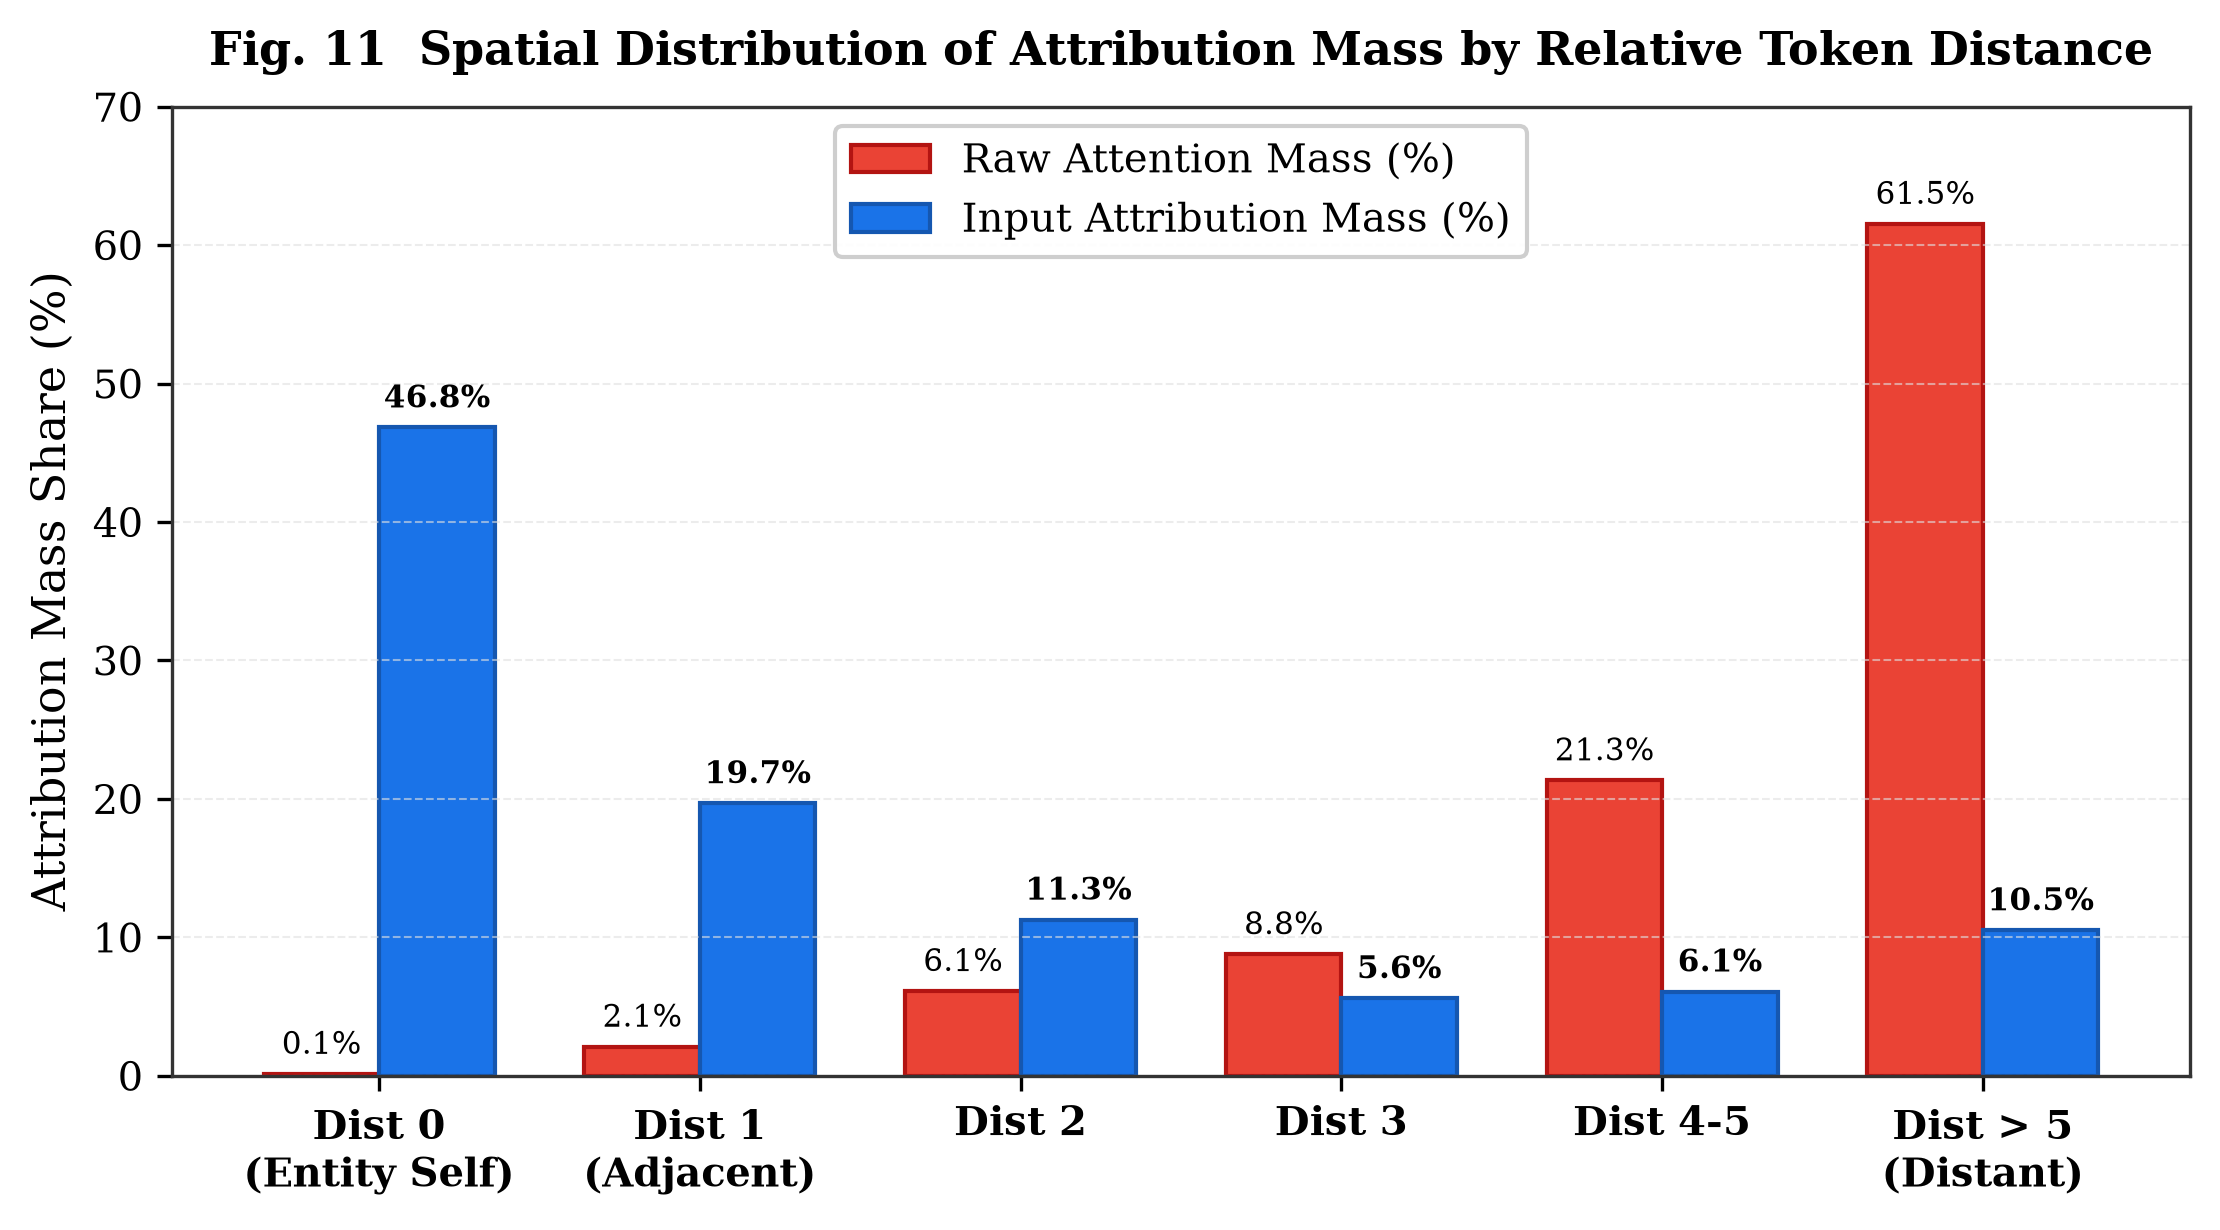
\includegraphics[width=0.48\textwidth]{figures/fig11_distance_distribution.png}
\caption{Attribution mass allocation across relative token distances, illustrating why attention behaves as a distant syntactic bus (61.5\% mass at dist $>5$) while input attribution concentrates on local context.}
\label{fig11}
\end{figure}

Raw attention assigns \textbf{61.53\% of its total probability mass to distant sentence tokens ($>5$ tokens away)}, primarily sentence delimiters, coordinating conjunctions, and root verbs. Because the preceding BiLSTM recurrent buffer contextualizes lexical tokens sequentially, the attention layer serves as a high-level broadcast bus rather than a feature selector. In contrast, input-level attribution allocates \textbf{77.80\% of its mass locally} (46.83\% on the entity itself and 30.97\% on immediate syntactic neighbors at distance 1--2), directly explaining its superior deletion faithfulness.

\begin{table}[h]
\caption{Integrated Gradients axiomatic completeness error across integration steps.}\label{tab12}
\centering
\begin{tabular}{lcccc}
\toprule
Steps ($m$) & Konkani Err & Assamese Err & Sinhala Err & Faithfulness Gap \\
\midrule
$m=10$ & 4.07\% & 4.37\% & 1.14\% & +0.1707 \\
$m=20$ & 2.05\% & 2.08\% & 0.56\% & +0.1799 \\
$m=50$ & \textbf{0.82\%} & \textbf{0.81\%} & \textbf{0.23\%} & \textbf{+0.1801} \\
\bottomrule
\end{tabular}
\end{table}

Table \ref{tab12} confirms that Integrated Gradients satisfies the completeness axiom with $<0.82\%$ relative error at 50 interpolation steps on the emission logit.

\section{Error Analysis and Qualitative Case Studies}\label{sec7}

Table \ref{tab15} illustrates representative success and failure cases identified during error analysis across all three languages.

\begin{table*}[t]
\caption{Qualitative case studies of attribution behavior on Gold-Dev.}\label{tab15}
\centering
\begin{tabular}{p{0.18\textwidth}p{0.32\textwidth}p{0.22\textwidth}p{0.20\textwidth}}
\toprule
Language / Class & Sentence Context & Attributed Context Tokens & Faithfulness Impact \\
\midrule
\textbf{Assamese} (`B-PER`) \textit{(Success)} & \textit{Dr. Himanta Biswa Sarma announced the new policy scheme.} & Top Context: `Dr.` (honorific title); Entity: `Himanta` & Erasing `Dr.` collapses PER marginal from 0.998 to 0.431 ($\text{Gap} = \mathbf{+0.565}$) \\
\textbf{Sinhala} (`B-LOC`) \textit{(Success)} & \textit{The summit was held in Colombo near Galle Face.} & Top Context: `in` (locative postposition `-di`); Entity: `Colombo` & Erasing locative marker drops LOC confidence by 0.784 ($\text{Gap} = \mathbf{+0.621}$) \\
\textbf{Konkani} (`B-MISC`) \textit{(Failure)} & \textit{In Mahabharata, Adiparva 167, according to the story...} & Top Context: `,` (comma delimiter); Entity: `Mahabharata` & Comma erasure causes zero drop; random erasure hits `Adiparva` ($\text{Gap} = \mathbf{-0.081}$) \\
\bottomrule
\end{tabular}
\end{table*}

Person entities (`PER`) exhibit massive context sensitivity (+0.6386 gap under input attribution) because South Asian honorific prefixes (`শ্রী`, `ডাঃ`, `ගරු`) serve as mandatory syntactic cues. Erasing an honorific immediately destroys entity recognition confidence. Conversely, miscellaneous entities (`MISC`) and locations (`LOC`) rely more heavily on autonomous lexical roots, resulting in moderate contextual gaps (+0.055 to +0.264).

\section{Limitations and Ethical Considerations}\label{sec8}

We explicitly delineate the epistemological boundaries of this study:
\begin{enumerate}
    \item \textbf{Deletion Faithfulness vs. Formal Causality}: Feature erasure evaluates deletion-based necessity under intervention \cite{hooker2019benchmark}. Zeroing input embeddings induces out-of-distribution (OOD) representation shifts. Our results establish superior deletion faithfulness, not formal Pearl counterfactual causality ($\text{do}$-calculus).
    \item \textbf{Exploratory Development-Set Evaluation}: Faithfulness benchmarks were conducted on Gold-Dev ($N=300$) to protect the Gold-Test benchmark from methodological peeking.
    \item \textbf{Sub-Category Sample Constraints}: Categories such as Sinhala `MISC` ($N=9$) and Assamese `ORG` ($N=15$) exhibit wider standard errors.
    \item \textbf{Environmental and Open Science Benefits}: Requiring zero external pretrained checkpoints achieves dramatic energy savings: the entire 4-stage pipeline trains in under 3.5 GPU hours on a single consumer laptop GPU ($<60\text{W}$ TDP).
\end{enumerate}

\section{Conclusion and Future Work}\label{sec9}

In this work, we presented a from-scratch neural Named Entity Recognition framework for Konkani, Assamese, and Sinhala, proving that strict architectural design (extended grapheme cluster tokenization, multi-filter Char-CNN, BiLSTM, multi-head self-attention, and linear-chain CRF) attains state-of-the-art accuracy without external pretrained models. The model achieves a Macro Entity F1 of \textbf{97.30\%} on locked Gold-Test splits, with 91.03\% out-of-vocabulary entity generalization. Through an independent, audited faithfulness benchmark, we resolved the attention interpretability debate in hybrid recurrent-attention models: raw self-attention functions as a broad syntactic broadcast bus (allocating 61.5\% of mass distantly), whereas input-level gradient attribution directly bypasses the BiLSTM buffer to provide highly faithful, localized explanations (+0.2449 gap, $p < 0.0001$). Future work will investigate counterfactual text generation and human-in-the-loop validation across additional indigenous languages.

\section*{Declarations}
\begin{itemize}
    \item \textbf{Funding}: No external funding was received for this research.
    \item \textbf{Conflict of Interest}: The authors declare no competing interests.
    \item \textbf{Data Availability}: All datasets, split manifests, and evaluation scripts are available in the project repository.
    \item \textbf{Code Availability}: All model definitions, training scripts, and explainability evaluation suites are publicly available.
\end{itemize}

\bibliography{references}

\end{document}
